\documentclass[]{article}
\usepackage{lmodern}
\usepackage{amssymb,amsmath}
\usepackage{ifxetex,ifluatex}
\usepackage{fixltx2e} % provides \textsubscript
\ifnum 0\ifxetex 1\fi\ifluatex 1\fi=0 % if pdftex
  \usepackage[T1]{fontenc}
  \usepackage[utf8]{inputenc}
\else % if luatex or xelatex
  \ifxetex
    \usepackage{mathspec}
  \else
    \usepackage{fontspec}
  \fi
  \defaultfontfeatures{Ligatures=TeX,Scale=MatchLowercase}
\fi
% use upquote if available, for straight quotes in verbatim environments
\IfFileExists{upquote.sty}{\usepackage{upquote}}{}
% use microtype if available
\IfFileExists{microtype.sty}{%
\usepackage{microtype}
\UseMicrotypeSet[protrusion]{basicmath} % disable protrusion for tt fonts
}{}
\usepackage[margin=1in]{geometry}
\usepackage{hyperref}
\hypersetup{unicode=true,
            pdftitle={IODS course project},
            pdfauthor={Ripsa Niemi},
            pdfborder={0 0 0},
            breaklinks=true}
\urlstyle{same}  % don't use monospace font for urls
\usepackage{color}
\usepackage{fancyvrb}
\newcommand{\VerbBar}{|}
\newcommand{\VERB}{\Verb[commandchars=\\\{\}]}
\DefineVerbatimEnvironment{Highlighting}{Verbatim}{commandchars=\\\{\}}
% Add ',fontsize=\small' for more characters per line
\usepackage{framed}
\definecolor{shadecolor}{RGB}{248,248,248}
\newenvironment{Shaded}{\begin{snugshade}}{\end{snugshade}}
\newcommand{\KeywordTok}[1]{\textcolor[rgb]{0.13,0.29,0.53}{\textbf{#1}}}
\newcommand{\DataTypeTok}[1]{\textcolor[rgb]{0.13,0.29,0.53}{#1}}
\newcommand{\DecValTok}[1]{\textcolor[rgb]{0.00,0.00,0.81}{#1}}
\newcommand{\BaseNTok}[1]{\textcolor[rgb]{0.00,0.00,0.81}{#1}}
\newcommand{\FloatTok}[1]{\textcolor[rgb]{0.00,0.00,0.81}{#1}}
\newcommand{\ConstantTok}[1]{\textcolor[rgb]{0.00,0.00,0.00}{#1}}
\newcommand{\CharTok}[1]{\textcolor[rgb]{0.31,0.60,0.02}{#1}}
\newcommand{\SpecialCharTok}[1]{\textcolor[rgb]{0.00,0.00,0.00}{#1}}
\newcommand{\StringTok}[1]{\textcolor[rgb]{0.31,0.60,0.02}{#1}}
\newcommand{\VerbatimStringTok}[1]{\textcolor[rgb]{0.31,0.60,0.02}{#1}}
\newcommand{\SpecialStringTok}[1]{\textcolor[rgb]{0.31,0.60,0.02}{#1}}
\newcommand{\ImportTok}[1]{#1}
\newcommand{\CommentTok}[1]{\textcolor[rgb]{0.56,0.35,0.01}{\textit{#1}}}
\newcommand{\DocumentationTok}[1]{\textcolor[rgb]{0.56,0.35,0.01}{\textbf{\textit{#1}}}}
\newcommand{\AnnotationTok}[1]{\textcolor[rgb]{0.56,0.35,0.01}{\textbf{\textit{#1}}}}
\newcommand{\CommentVarTok}[1]{\textcolor[rgb]{0.56,0.35,0.01}{\textbf{\textit{#1}}}}
\newcommand{\OtherTok}[1]{\textcolor[rgb]{0.56,0.35,0.01}{#1}}
\newcommand{\FunctionTok}[1]{\textcolor[rgb]{0.00,0.00,0.00}{#1}}
\newcommand{\VariableTok}[1]{\textcolor[rgb]{0.00,0.00,0.00}{#1}}
\newcommand{\ControlFlowTok}[1]{\textcolor[rgb]{0.13,0.29,0.53}{\textbf{#1}}}
\newcommand{\OperatorTok}[1]{\textcolor[rgb]{0.81,0.36,0.00}{\textbf{#1}}}
\newcommand{\BuiltInTok}[1]{#1}
\newcommand{\ExtensionTok}[1]{#1}
\newcommand{\PreprocessorTok}[1]{\textcolor[rgb]{0.56,0.35,0.01}{\textit{#1}}}
\newcommand{\AttributeTok}[1]{\textcolor[rgb]{0.77,0.63,0.00}{#1}}
\newcommand{\RegionMarkerTok}[1]{#1}
\newcommand{\InformationTok}[1]{\textcolor[rgb]{0.56,0.35,0.01}{\textbf{\textit{#1}}}}
\newcommand{\WarningTok}[1]{\textcolor[rgb]{0.56,0.35,0.01}{\textbf{\textit{#1}}}}
\newcommand{\AlertTok}[1]{\textcolor[rgb]{0.94,0.16,0.16}{#1}}
\newcommand{\ErrorTok}[1]{\textcolor[rgb]{0.64,0.00,0.00}{\textbf{#1}}}
\newcommand{\NormalTok}[1]{#1}
\usepackage{graphicx,grffile}
\makeatletter
\def\maxwidth{\ifdim\Gin@nat@width>\linewidth\linewidth\else\Gin@nat@width\fi}
\def\maxheight{\ifdim\Gin@nat@height>\textheight\textheight\else\Gin@nat@height\fi}
\makeatother
% Scale images if necessary, so that they will not overflow the page
% margins by default, and it is still possible to overwrite the defaults
% using explicit options in \includegraphics[width, height, ...]{}
\setkeys{Gin}{width=\maxwidth,height=\maxheight,keepaspectratio}
\IfFileExists{parskip.sty}{%
\usepackage{parskip}
}{% else
\setlength{\parindent}{0pt}
\setlength{\parskip}{6pt plus 2pt minus 1pt}
}
\setlength{\emergencystretch}{3em}  % prevent overfull lines
\providecommand{\tightlist}{%
  \setlength{\itemsep}{0pt}\setlength{\parskip}{0pt}}
\setcounter{secnumdepth}{0}
% Redefines (sub)paragraphs to behave more like sections
\ifx\paragraph\undefined\else
\let\oldparagraph\paragraph
\renewcommand{\paragraph}[1]{\oldparagraph{#1}\mbox{}}
\fi
\ifx\subparagraph\undefined\else
\let\oldsubparagraph\subparagraph
\renewcommand{\subparagraph}[1]{\oldsubparagraph{#1}\mbox{}}
\fi

%%% Use protect on footnotes to avoid problems with footnotes in titles
\let\rmarkdownfootnote\footnote%
\def\footnote{\protect\rmarkdownfootnote}

%%% Change title format to be more compact
\usepackage{titling}

% Create subtitle command for use in maketitle
\providecommand{\subtitle}[1]{
  \posttitle{
    \begin{center}\large#1\end{center}
    }
}

\setlength{\droptitle}{-2em}

  \title{IODS course project}
    \pretitle{\vspace{\droptitle}\centering\huge}
  \posttitle{\par}
    \author{Ripsa Niemi}
    \preauthor{\centering\large\emph}
  \postauthor{\par}
    \date{}
    \predate{}\postdate{}
  

\begin{document}
\maketitle

{
\setcounter{tocdepth}{2}
\tableofcontents
}
\begin{center}\rule{0.5\linewidth}{\linethickness}\end{center}

\section{About the project}\label{about-the-project}

This is a project done in University of Helsinki in a course
\textbf{Introduction to Open Data Science} during Fall 2019. Project
includes different statistical methods, tests and visualizations used to
different open source datasets.

During this course I became more comfortable using R and it's packages.
It became one of my favorite courses of all time! I was really excited
about doing analyses with different data sets and also learning how to
visualize and wrangle data better.

My GitHub repository
\href{https://github.com/ripsaniemi/IODS-project}{can be found here}.

\begin{center}\rule{0.5\linewidth}{\linethickness}\end{center}

\section{Week 2: Linear regression}\label{week-2-linear-regression}

\subsubsection{1)}\label{section}

\subsubsection{Exploring the datasets of the
week}\label{exploring-the-datasets-of-the-week}

\begin{Shaded}
\begin{Highlighting}[]
\NormalTok{data <-}\StringTok{ }\KeywordTok{read.csv}\NormalTok{(}\StringTok{"data/learning2014.csv"}\NormalTok{)}

\KeywordTok{head}\NormalTok{(data)}
\end{Highlighting}
\end{Shaded}

\begin{verbatim}
##   gender age attitude     deep  stra     surf points
## 1      F  53       37 3.583333 3.375 2.583333     25
## 2      M  55       31 2.916667 2.750 3.166667     12
## 3      F  49       25 3.500000 3.625 2.250000     24
## 4      M  53       35 3.500000 3.125 2.250000     10
## 5      M  49       37 3.666667 3.625 2.833333     22
## 6      F  38       38 4.750000 3.625 2.416667     21
\end{verbatim}

\begin{Shaded}
\begin{Highlighting}[]
\KeywordTok{str}\NormalTok{(data)}
\end{Highlighting}
\end{Shaded}

\begin{verbatim}
## 'data.frame':    166 obs. of  7 variables:
##  $ gender  : Factor w/ 2 levels "F","M": 1 2 1 2 2 1 2 1 2 1 ...
##  $ age     : int  53 55 49 53 49 38 50 37 37 42 ...
##  $ attitude: int  37 31 25 35 37 38 35 29 38 21 ...
##  $ deep    : num  3.58 2.92 3.5 3.5 3.67 ...
##  $ stra    : num  3.38 2.75 3.62 3.12 3.62 ...
##  $ surf    : num  2.58 3.17 2.25 2.25 2.83 ...
##  $ points  : int  25 12 24 10 22 21 21 31 24 26 ...
\end{verbatim}

This data was collected from students of course Introduction to Social
Statistics, fall 2014.\\
Data has \textbf{166 observations and 7 variables}:

\begin{itemize}
\tightlist
\item
  gender (M/F),\\
\item
  age,\\
\item
  attitude (Global attitude toward statistics),
\item
  deep (mean of ``deep approach'' questions measuring seeking meaning,
  relating ideas and use of evidence)
\item
  stra (mean of ``Strategic approach'' questions measuring organized
  studying and time management)
\item
  surf (mean of ``Surface approach'' questions measuring Lack of
  purpose, Unrelated memorising, sullabys-boudness)
\item
  points (Exam points)
\end{itemize}

\subsubsection{2)}\label{section-1}

\subsubsection{Summary and relationships between
variables}\label{summary-and-relationships-between-variables}

\begin{Shaded}
\begin{Highlighting}[]
\KeywordTok{library}\NormalTok{(ggplot2)}
\KeywordTok{library}\NormalTok{(GGally)}
\end{Highlighting}
\end{Shaded}

\begin{verbatim}
## Registered S3 method overwritten by 'GGally':
##   method from   
##   +.gg   ggplot2
\end{verbatim}

\begin{Shaded}
\begin{Highlighting}[]
\NormalTok{g1 <-}\StringTok{ }\KeywordTok{ggpairs}\NormalTok{(data, }\KeywordTok{aes}\NormalTok{(}\DataTypeTok{color =}\NormalTok{ gender)) }\OperatorTok{+}\StringTok{ }
\StringTok{  }\KeywordTok{ggtitle}\NormalTok{(}\StringTok{"Scatterplot matrix"}\NormalTok{)}

\NormalTok{g1}
\end{Highlighting}
\end{Shaded}

\begin{verbatim}
## `stat_bin()` using `bins = 30`. Pick better value with `binwidth`.
\end{verbatim}

\begin{verbatim}
## `stat_bin()` using `bins = 30`. Pick better value with `binwidth`.
## `stat_bin()` using `bins = 30`. Pick better value with `binwidth`.
## `stat_bin()` using `bins = 30`. Pick better value with `binwidth`.
## `stat_bin()` using `bins = 30`. Pick better value with `binwidth`.
## `stat_bin()` using `bins = 30`. Pick better value with `binwidth`.
\end{verbatim}

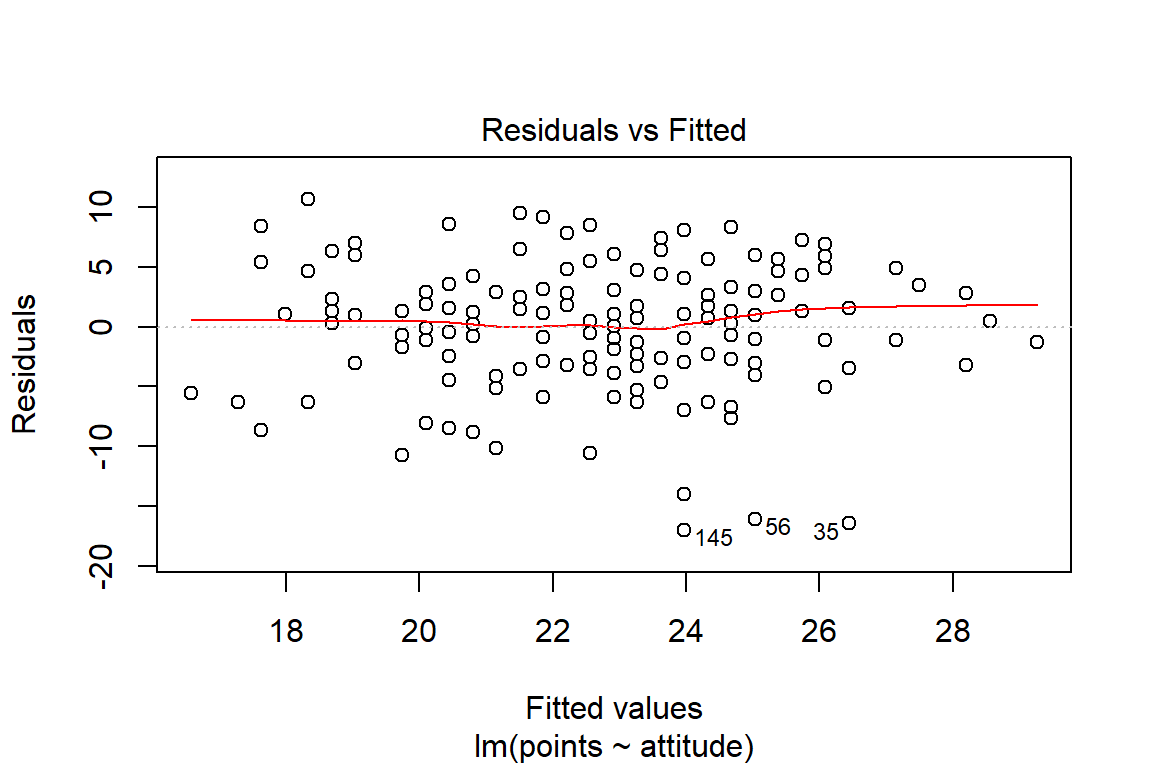
\includegraphics{index_files/figure-latex/unnamed-chunk-8-1.pdf}

\begin{Shaded}
\begin{Highlighting}[]
\KeywordTok{summary}\NormalTok{(data)}
\end{Highlighting}
\end{Shaded}

\begin{verbatim}
##  gender       age           attitude          deep            stra      
##  F:110   Min.   :17.00   Min.   :14.00   Min.   :1.583   Min.   :1.250  
##  M: 56   1st Qu.:21.00   1st Qu.:26.00   1st Qu.:3.333   1st Qu.:2.625  
##          Median :22.00   Median :32.00   Median :3.667   Median :3.188  
##          Mean   :25.51   Mean   :31.43   Mean   :3.680   Mean   :3.121  
##          3rd Qu.:27.00   3rd Qu.:37.00   3rd Qu.:4.083   3rd Qu.:3.625  
##          Max.   :55.00   Max.   :50.00   Max.   :4.917   Max.   :5.000  
##       surf           points     
##  Min.   :1.583   Min.   : 7.00  
##  1st Qu.:2.417   1st Qu.:19.00  
##  Median :2.833   Median :23.00  
##  Mean   :2.787   Mean   :22.72  
##  3rd Qu.:3.167   3rd Qu.:27.75  
##  Max.   :4.333   Max.   :33.00
\end{verbatim}

Trough the scatter plot we can easily study how the data and variables
look like. Red means female and blue male observations. Biggest
difference between genders seems to be on variable attitude, where
females have a clearly lower mean.

Highest (absolute) correlations are between variables points - attitude,
deep - surf and surf - stra.

Summary function shows us that approximately 2/3 of people answering the
survey are female. Mean age of pariticipants is 25.5 years old and mean
points from exam was 22.7 and mean on attitude 31.4.

\subsubsection{3)}\label{section-2}

\subsubsection{Finding explanatory variables to
Points}\label{finding-explanatory-variables-to-points}

We see that the three variables that have the highest (absolute)
correlation with points are attitude, stra and surf. Lets start with a
linear regression with those three as explanatory variables:

\begin{Shaded}
\begin{Highlighting}[]
\NormalTok{r1 <-}\StringTok{ }\KeywordTok{lm}\NormalTok{(points }\OperatorTok{~}\StringTok{ }\NormalTok{attitude }\OperatorTok{+}\StringTok{ }\NormalTok{stra }\OperatorTok{+}\StringTok{ }\NormalTok{surf, }\DataTypeTok{data =}\NormalTok{ data)}
\KeywordTok{summary}\NormalTok{(r1)}
\end{Highlighting}
\end{Shaded}

\begin{verbatim}
## 
## Call:
## lm(formula = points ~ attitude + stra + surf, data = data)
## 
## Residuals:
##      Min       1Q   Median       3Q      Max 
## -17.1550  -3.4346   0.5156   3.6401  10.8952 
## 
## Coefficients:
##             Estimate Std. Error t value Pr(>|t|)    
## (Intercept) 11.01711    3.68375   2.991  0.00322 ** 
## attitude     0.33952    0.05741   5.913 1.93e-08 ***
## stra         0.85313    0.54159   1.575  0.11716    
## surf        -0.58607    0.80138  -0.731  0.46563    
## ---
## Signif. codes:  0 '***' 0.001 '**' 0.01 '*' 0.05 '.' 0.1 ' ' 1
## 
## Residual standard error: 5.296 on 162 degrees of freedom
## Multiple R-squared:  0.2074, Adjusted R-squared:  0.1927 
## F-statistic: 14.13 on 3 and 162 DF,  p-value: 3.156e-08
\end{verbatim}

Our p-value is 3.125e-08, so this there is statistically significant
relationship between explanatory variables and points. In this model
alpha would be 11.02, beeta1 0.34, beeta2 0.85 and beeta3 -0.59.

However, when we look at these three variabes only one of them,
attitude, has a statistically significant p-value = 1.93e-08
(\textless{}0.05). For this reason, let's take stra and surf out of the
regression, since we can conclude that they are not making this model
any better.

\subsubsection{4)}\label{section-3}

\subsubsection{Linear regression with points as dependent variable and
attitude as explanatory
variable}\label{linear-regression-with-points-as-dependent-variable-and-attitude-as-explanatory-variable}

\begin{Shaded}
\begin{Highlighting}[]
\NormalTok{r2 <-}\StringTok{ }\KeywordTok{lm}\NormalTok{(points }\OperatorTok{~}\StringTok{ }\NormalTok{attitude, data)}
\KeywordTok{summary}\NormalTok{(r2)}
\end{Highlighting}
\end{Shaded}

\begin{verbatim}
## 
## Call:
## lm(formula = points ~ attitude, data = data)
## 
## Residuals:
##      Min       1Q   Median       3Q      Max 
## -16.9763  -3.2119   0.4339   4.1534  10.6645 
## 
## Coefficients:
##             Estimate Std. Error t value Pr(>|t|)    
## (Intercept) 11.63715    1.83035   6.358 1.95e-09 ***
## attitude     0.35255    0.05674   6.214 4.12e-09 ***
## ---
## Signif. codes:  0 '***' 0.001 '**' 0.01 '*' 0.05 '.' 0.1 ' ' 1
## 
## Residual standard error: 5.32 on 164 degrees of freedom
## Multiple R-squared:  0.1906, Adjusted R-squared:  0.1856 
## F-statistic: 38.61 on 1 and 164 DF,  p-value: 4.119e-09
\end{verbatim}

\begin{Shaded}
\begin{Highlighting}[]
\NormalTok{g2 <-}\StringTok{ }\KeywordTok{ggplot}\NormalTok{(data, }\KeywordTok{aes}\NormalTok{(}\DataTypeTok{x =}\NormalTok{ attitude, }\DataTypeTok{y =}\NormalTok{ points)) }\OperatorTok{+}\StringTok{ }\KeywordTok{geom_point}\NormalTok{() }\OperatorTok{+}\StringTok{ }\KeywordTok{ggtitle}\NormalTok{(}\StringTok{"Linear regression of points and attitude"}\NormalTok{) }\OperatorTok{+}\StringTok{ }\KeywordTok{geom_smooth}\NormalTok{(}\DataTypeTok{method =} \StringTok{"lm"}\NormalTok{)}
\NormalTok{g2}
\end{Highlighting}
\end{Shaded}

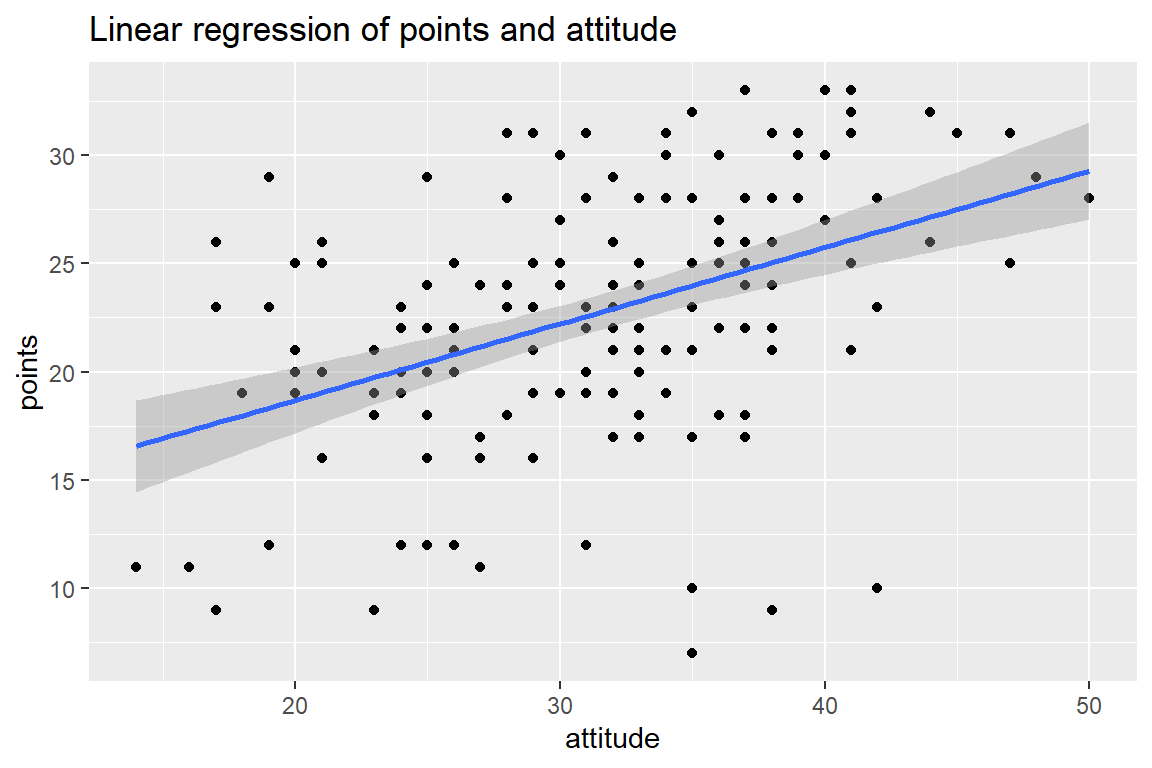
\includegraphics{index_files/figure-latex/unnamed-chunk-10-1.pdf}
P-value is 4.119e-09, so this the relationship is statistically
significant.

If we would want to predict values of points using variable attitude,
the model would be\\
y = 11.63715 + 0.35255x\\
where y is points and x attitude.

This means that when attitude increases, points increases as well. This
result can be seen through the scatterplot where the regression line is
drawn.

R-squared is 0.19, which means that this model explains 19\% of the
variation of dependent variable Points.

\subsubsection{5)}\label{section-4}

\subsubsection{Diagnostic plots and graphical model
validation}\label{diagnostic-plots-and-graphical-model-validation}

\begin{Shaded}
\begin{Highlighting}[]
\KeywordTok{plot}\NormalTok{(r2, }\DataTypeTok{which =} \DecValTok{1}\NormalTok{)}
\end{Highlighting}
\end{Shaded}

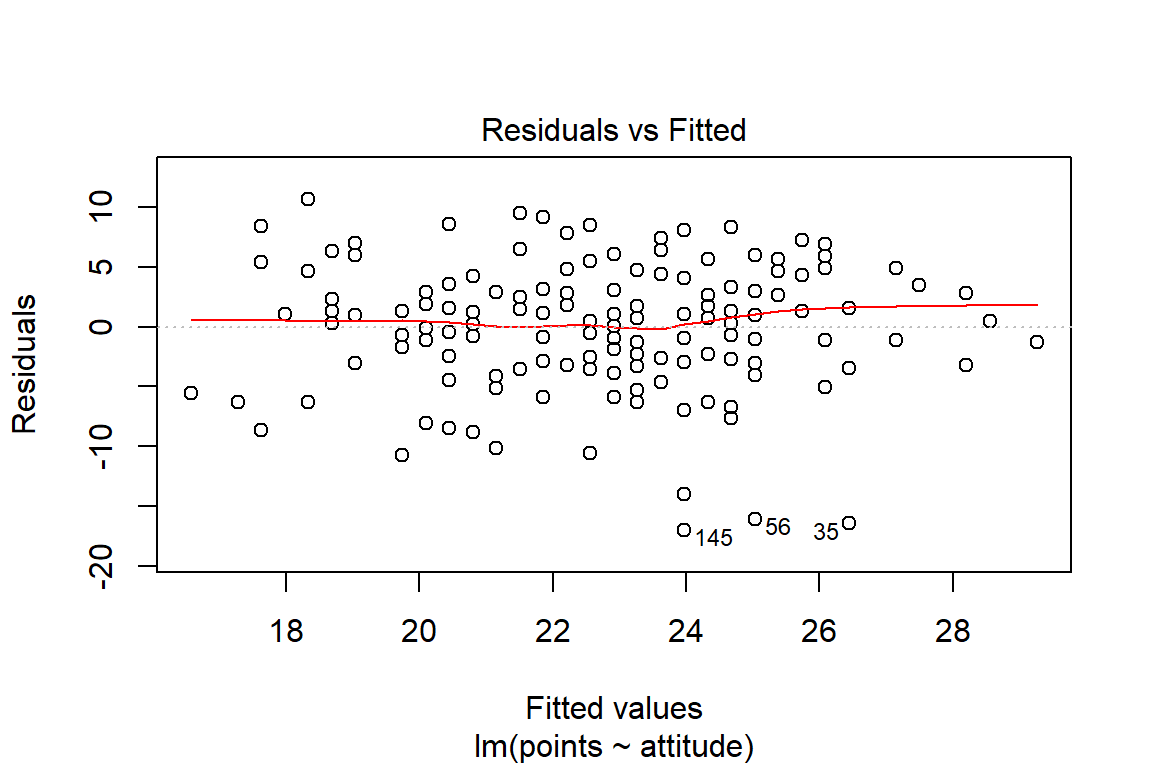
\includegraphics{index_files/figure-latex/unnamed-chunk-11-1.pdf}

\begin{Shaded}
\begin{Highlighting}[]
\KeywordTok{plot}\NormalTok{(r2, }\DataTypeTok{which =} \DecValTok{2}\NormalTok{)}
\end{Highlighting}
\end{Shaded}

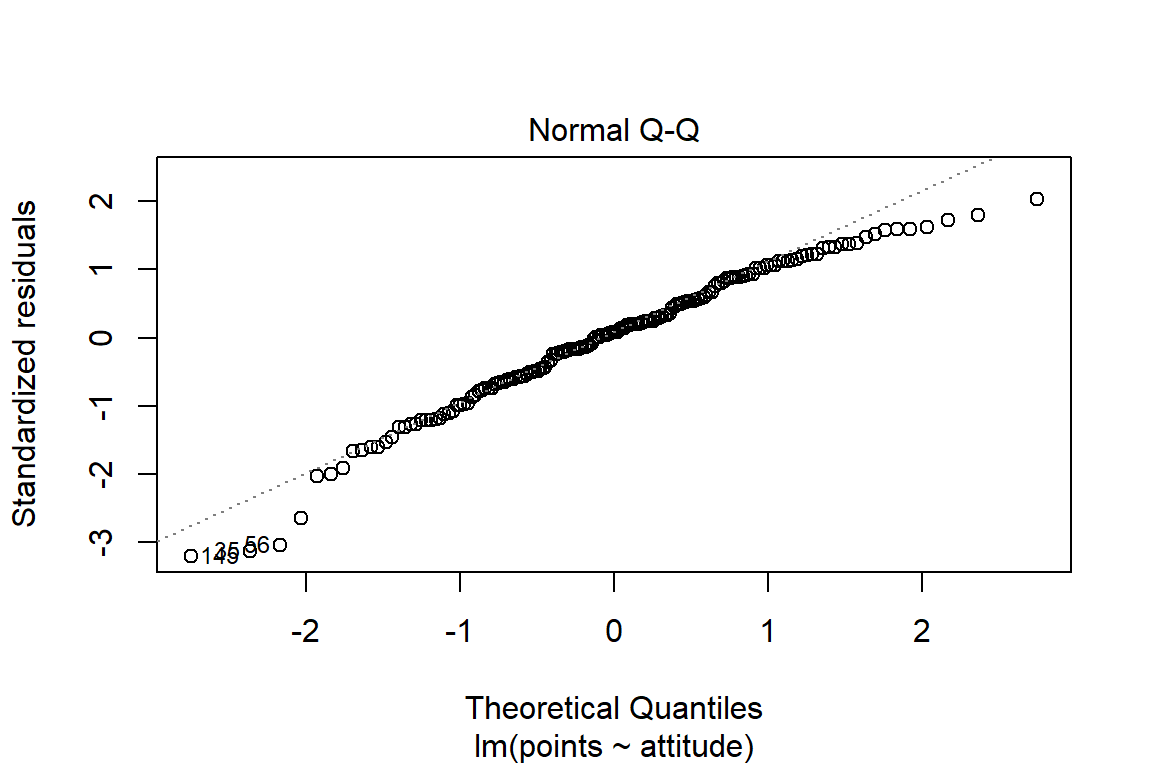
\includegraphics{index_files/figure-latex/unnamed-chunk-11-2.pdf}

\begin{Shaded}
\begin{Highlighting}[]
\KeywordTok{plot}\NormalTok{(r2, }\DataTypeTok{which =} \DecValTok{5}\NormalTok{)}
\end{Highlighting}
\end{Shaded}

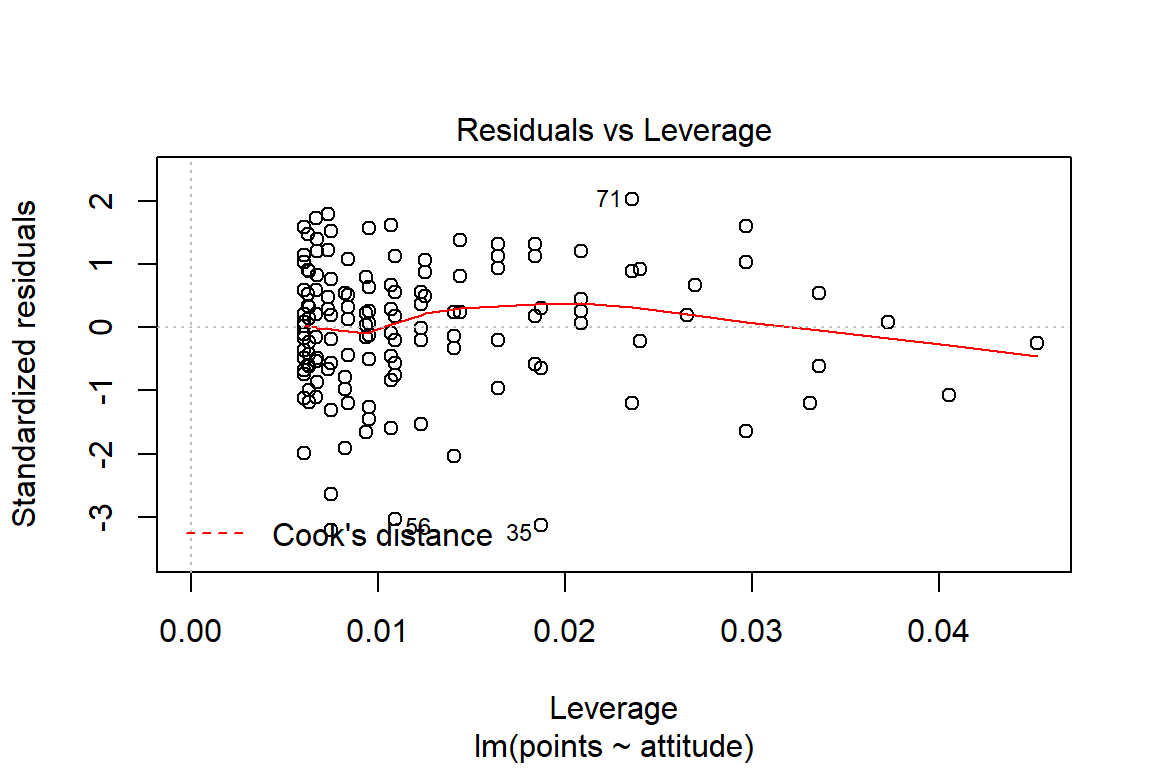
\includegraphics{index_files/figure-latex/unnamed-chunk-11-3.pdf}

When we use linear regression we assume that the relationship between x
and y is linear. We also assume that the errors are normally distributed
and varince is constant: so the errors do not depend on explanatory
variable.

Residuals vs Fitted values shows whether variance is constant. Although
the points seem to be pretty randomly spread at first, there is a small
pattern where on right side the points are not as spread as on the left
side. This implies a problem.

Normal QQ-plot shows us how well the errors are normally distributed.
The better the points are in the line, the better we can asumme this.
Normal QQ is reasonable, but not perfect, since on both ends the points
deviate from the a bit too much. This might be a problem as well.

Residuals vs Leverage shows whether there are observations, that have a
high impact on the model. This seems to be okay, so no data point has an
exteremely high leverage.

\begin{center}\rule{0.5\linewidth}{\linethickness}\end{center}

\section{Week 3: Logistic regression}\label{week-3-logistic-regression}

\subsection{1) Starting the week}\label{starting-the-week}

This week we learn to do logistic regression, first let's read the
datasets and have a look at it.

\subsection{2) Reading the datasets}\label{reading-the-datasets}

\begin{Shaded}
\begin{Highlighting}[]
\KeywordTok{library}\NormalTok{(dplyr); }\KeywordTok{library}\NormalTok{(ggplot2)}
\end{Highlighting}
\end{Shaded}

\begin{verbatim}
## 
## Attaching package: 'dplyr'
\end{verbatim}

\begin{verbatim}
## The following object is masked from 'package:GGally':
## 
##     nasa
\end{verbatim}

\begin{verbatim}
## The following objects are masked from 'package:stats':
## 
##     filter, lag
\end{verbatim}

\begin{verbatim}
## The following objects are masked from 'package:base':
## 
##     intersect, setdiff, setequal, union
\end{verbatim}

\begin{Shaded}
\begin{Highlighting}[]
\NormalTok{alc <-}\StringTok{ }\KeywordTok{read.csv}\NormalTok{(}\StringTok{"data/alc.csv"}\NormalTok{)}

\KeywordTok{glimpse}\NormalTok{(alc)}
\end{Highlighting}
\end{Shaded}

\begin{verbatim}
## Observations: 382
## Variables: 35
## $ school     <fct> GP, GP, GP, GP, GP, GP, GP, GP, GP, GP, GP, GP, GP,...
## $ sex        <fct> F, F, F, F, F, M, M, F, M, M, F, F, M, M, M, F, F, ...
## $ age        <int> 18, 17, 15, 15, 16, 16, 16, 17, 15, 15, 15, 15, 15,...
## $ address    <fct> U, U, U, U, U, U, U, U, U, U, U, U, U, U, U, U, U, ...
## $ famsize    <fct> GT3, GT3, LE3, GT3, GT3, LE3, LE3, GT3, LE3, GT3, G...
## $ Pstatus    <fct> A, T, T, T, T, T, T, A, A, T, T, T, T, T, A, T, T, ...
## $ Medu       <int> 4, 1, 1, 4, 3, 4, 2, 4, 3, 3, 4, 2, 4, 4, 2, 4, 4, ...
## $ Fedu       <int> 4, 1, 1, 2, 3, 3, 2, 4, 2, 4, 4, 1, 4, 3, 2, 4, 4, ...
## $ Mjob       <fct> at_home, at_home, at_home, health, other, services,...
## $ Fjob       <fct> teacher, other, other, services, other, other, othe...
## $ reason     <fct> course, course, other, home, home, reputation, home...
## $ nursery    <fct> yes, no, yes, yes, yes, yes, yes, yes, yes, yes, ye...
## $ internet   <fct> no, yes, yes, yes, no, yes, yes, no, yes, yes, yes,...
## $ guardian   <fct> mother, father, mother, mother, father, mother, mot...
## $ traveltime <int> 2, 1, 1, 1, 1, 1, 1, 2, 1, 1, 1, 3, 1, 2, 1, 1, 1, ...
## $ studytime  <int> 2, 2, 2, 3, 2, 2, 2, 2, 2, 2, 2, 3, 1, 2, 3, 1, 3, ...
## $ failures   <int> 0, 0, 2, 0, 0, 0, 0, 0, 0, 0, 0, 0, 0, 0, 0, 0, 0, ...
## $ schoolsup  <fct> yes, no, yes, no, no, no, no, yes, no, no, no, no, ...
## $ famsup     <fct> no, yes, no, yes, yes, yes, no, yes, yes, yes, yes,...
## $ paid       <fct> no, no, yes, yes, yes, yes, no, no, yes, yes, yes, ...
## $ activities <fct> no, no, no, yes, no, yes, no, no, no, yes, no, yes,...
## $ higher     <fct> yes, yes, yes, yes, yes, yes, yes, yes, yes, yes, y...
## $ romantic   <fct> no, no, no, yes, no, no, no, no, no, no, no, no, no...
## $ famrel     <int> 4, 5, 4, 3, 4, 5, 4, 4, 4, 5, 3, 5, 4, 5, 4, 4, 3, ...
## $ freetime   <int> 3, 3, 3, 2, 3, 4, 4, 1, 2, 5, 3, 2, 3, 4, 5, 4, 2, ...
## $ goout      <int> 4, 3, 2, 2, 2, 2, 4, 4, 2, 1, 3, 2, 3, 3, 2, 4, 3, ...
## $ Dalc       <int> 1, 1, 2, 1, 1, 1, 1, 1, 1, 1, 1, 1, 1, 1, 1, 1, 1, ...
## $ Walc       <int> 1, 1, 3, 1, 2, 2, 1, 1, 1, 1, 2, 1, 3, 2, 1, 2, 2, ...
## $ health     <int> 3, 3, 3, 5, 5, 5, 3, 1, 1, 5, 2, 4, 5, 3, 3, 2, 2, ...
## $ absences   <int> 5, 3, 8, 1, 2, 8, 0, 4, 0, 0, 1, 2, 1, 1, 0, 5, 8, ...
## $ G1         <int> 2, 7, 10, 14, 8, 14, 12, 8, 16, 13, 12, 10, 13, 11,...
## $ G2         <int> 8, 8, 10, 14, 12, 14, 12, 9, 17, 14, 11, 12, 14, 11...
## $ G3         <int> 8, 8, 11, 14, 12, 14, 12, 10, 18, 14, 12, 12, 13, 1...
## $ alc_use    <dbl> 1.0, 1.0, 2.5, 1.0, 1.5, 1.5, 1.0, 1.0, 1.0, 1.0, 1...
## $ high_use   <lgl> FALSE, FALSE, TRUE, FALSE, FALSE, FALSE, FALSE, FAL...
\end{verbatim}

This dataset has 35 variables and 382 observations. It was collected
from two Portuguese secondary education schools and has variables about
socio-economical background, studying and free time.

I added two variables to dataset: alc\_use, which is a mean of daily and
weekend alcolhol use (Dalc, Walc) and high\_use, which is a binary
variable, True if alc\_use is over 2, False otherwise. I am using the
variable high use as the explained varible y in my logistic regression.

\subsection{3) Personal hypothesis of relationships with high/low
alcohol use and 4
variables}\label{personal-hypothesis-of-relationships-with-highlow-alcohol-use-and-4-variables}

I am choosing my prediction variables as goout, studytime, absences and
higher.

My personal hypothesis is that going out (goout) and having absences at
school affect high\_use positively, so high numbers imply True High
alcohol use.

Studytime and wanting to go to a higher education (higher) affect
high\_use negatively, so high numbers in studytime and yes in higher
imply False in High alcohol use.

\subsection{4) Numerical \& graphical exploration of the variable
distributions and relationship with
high\_use}\label{numerical-graphical-exploration-of-the-variable-distributions-and-relationship-with-high_use}

\begin{Shaded}
\begin{Highlighting}[]
\NormalTok{g <-}\StringTok{ }\KeywordTok{ggplot}\NormalTok{(}\DataTypeTok{data =}\NormalTok{ alc, }\KeywordTok{aes}\NormalTok{(}\DataTypeTok{x =}\NormalTok{ high_use, }\DataTypeTok{y =}\NormalTok{ studytime, }\DataTypeTok{col =}\NormalTok{ sex))}
\NormalTok{g  }\OperatorTok{+}\StringTok{ }\KeywordTok{geom_boxplot}\NormalTok{() }\OperatorTok{+}\StringTok{ }\KeywordTok{ggtitle}\NormalTok{(}\StringTok{"Studytime and high use"}\NormalTok{)}
\end{Highlighting}
\end{Shaded}

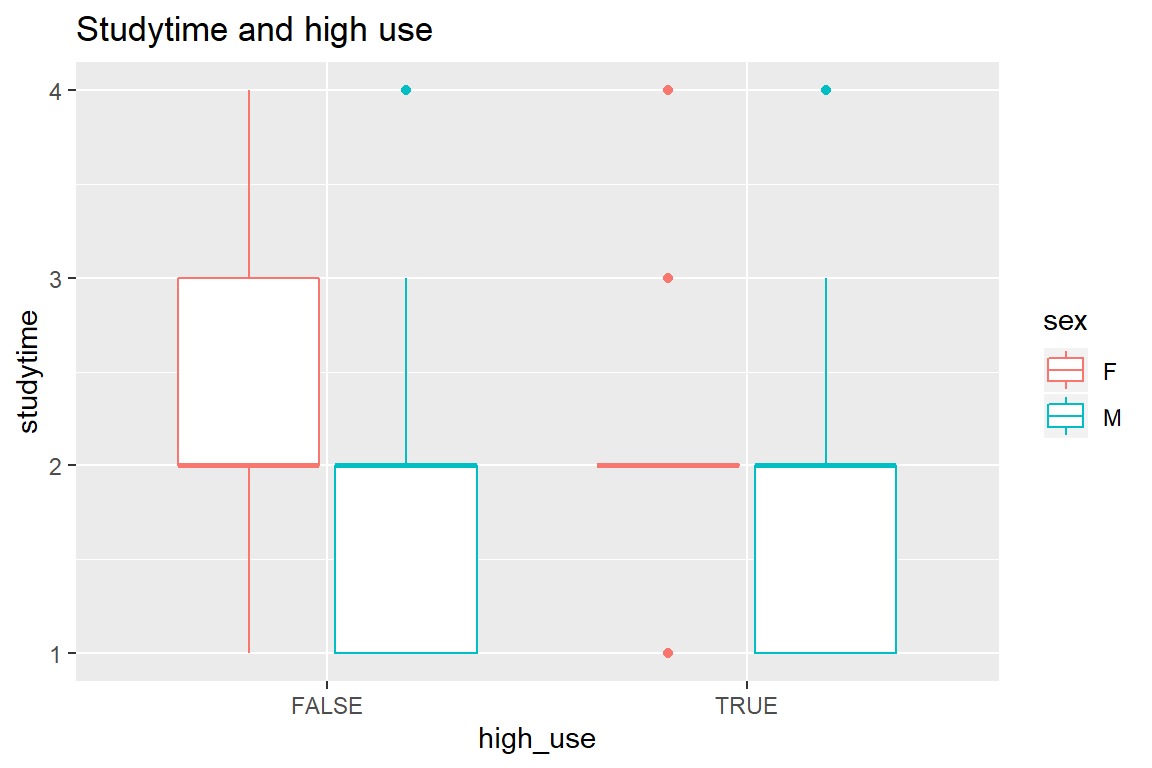
\includegraphics{index_files/figure-latex/unnamed-chunk-13-1.pdf}

\begin{Shaded}
\begin{Highlighting}[]
\KeywordTok{table}\NormalTok{(alc}\OperatorTok{$}\NormalTok{high_use, alc}\OperatorTok{$}\NormalTok{higher)}
\end{Highlighting}
\end{Shaded}

\begin{verbatim}
##        
##          no yes
##   FALSE   9 259
##   TRUE    9 105
\end{verbatim}

\begin{Shaded}
\begin{Highlighting}[]
\NormalTok{g2 <-}\StringTok{ }\KeywordTok{ggplot}\NormalTok{(}\DataTypeTok{data =}\NormalTok{ alc, }\KeywordTok{aes}\NormalTok{(}\DataTypeTok{x =}\NormalTok{ high_use, }\DataTypeTok{y =}\NormalTok{ goout, }\DataTypeTok{col =}\NormalTok{ sex)) }
\NormalTok{g2 }\OperatorTok{+}\StringTok{ }\KeywordTok{geom_boxplot}\NormalTok{() }\OperatorTok{+}\StringTok{ }\KeywordTok{ggtitle}\NormalTok{(}\StringTok{"Going out and high use"}\NormalTok{)}
\end{Highlighting}
\end{Shaded}

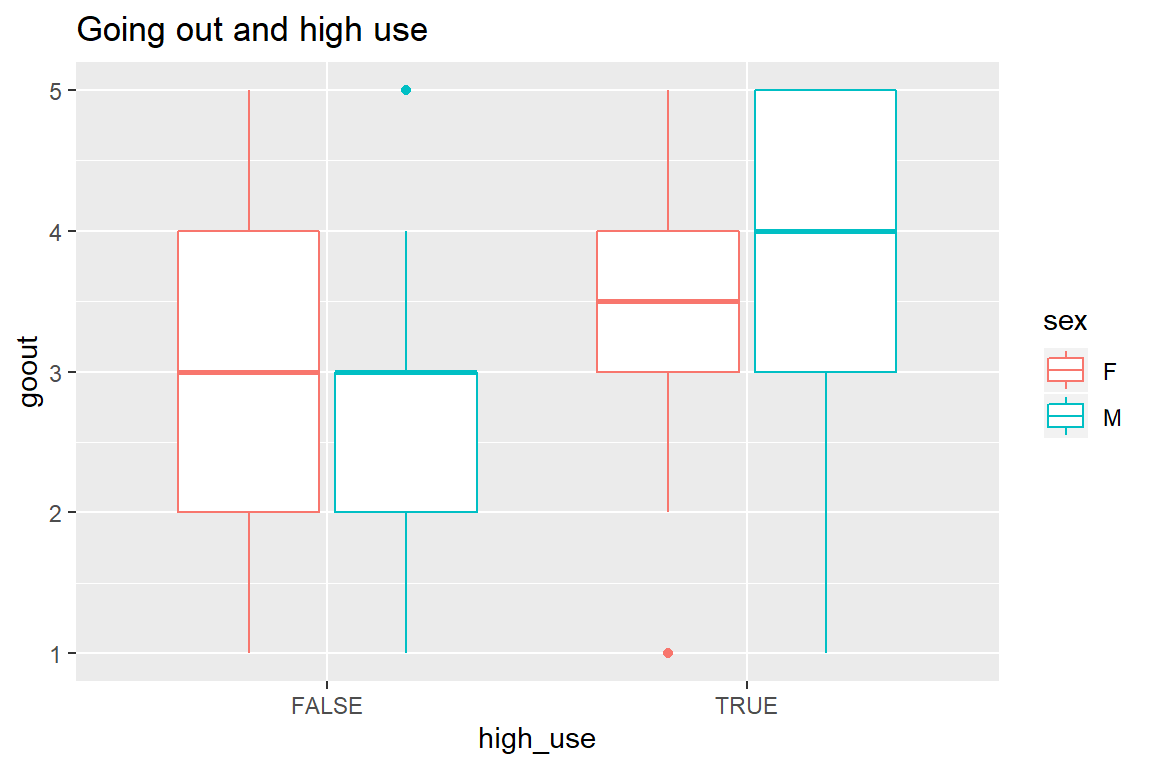
\includegraphics{index_files/figure-latex/unnamed-chunk-13-2.pdf}

\begin{Shaded}
\begin{Highlighting}[]
\NormalTok{g3 <-}\StringTok{ }\KeywordTok{ggplot}\NormalTok{(}\DataTypeTok{data =}\NormalTok{ alc, }\KeywordTok{aes}\NormalTok{(}\DataTypeTok{x =}\NormalTok{ high_use, }\DataTypeTok{y =}\NormalTok{ absences, }\DataTypeTok{col =}\NormalTok{ sex )) }
\NormalTok{g3 }\OperatorTok{+}\StringTok{  }\KeywordTok{geom_boxplot}\NormalTok{() }\OperatorTok{+}\StringTok{ }\KeywordTok{ggtitle}\NormalTok{(}\StringTok{"Absences and high use"}\NormalTok{)}
\end{Highlighting}
\end{Shaded}

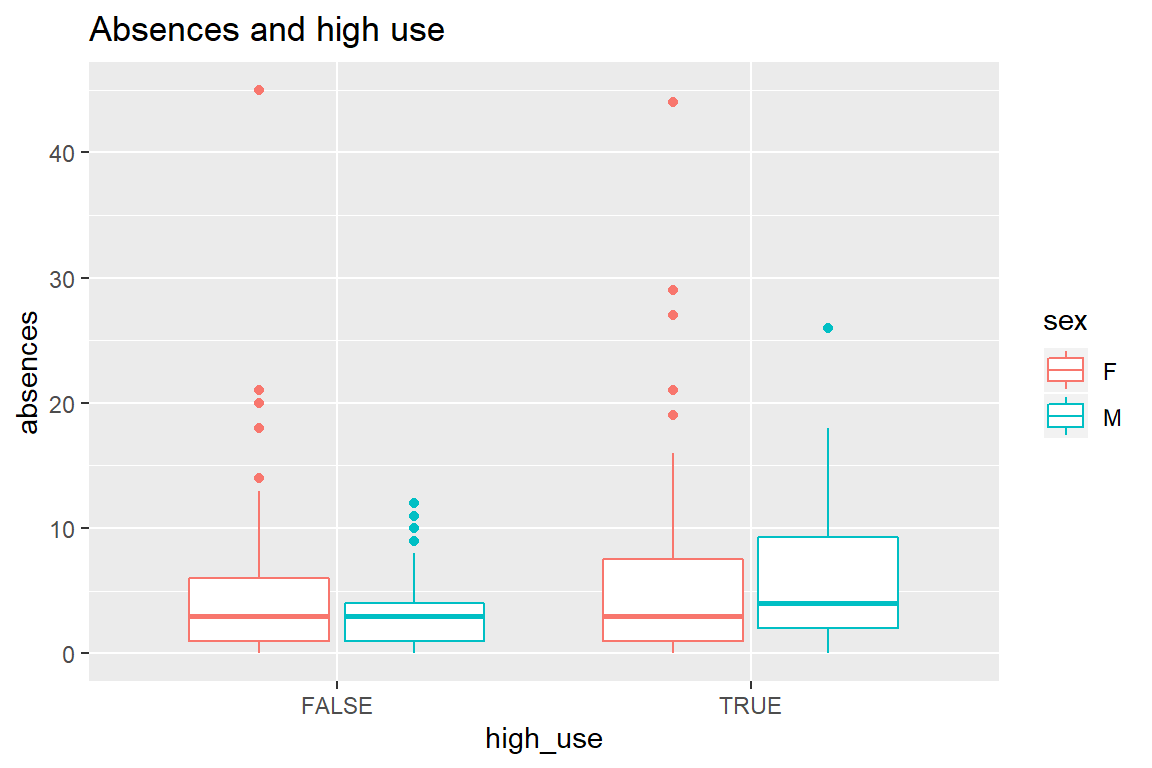
\includegraphics{index_files/figure-latex/unnamed-chunk-13-3.pdf}

Now let's look at these boxplots and table.

\textbf{Studytime and high use:} Studytime seems to be longer among
females, who are not high users. Among males studytime seems to have no
relationship with high use.

\textbf{Higher education goals and high use:} Those who said they wish
to have higher education are more often not high users (over two times).
However not wanting a higher education is not connected to high use, and
with small n is hard to say anything at all.

\textbf{Going out and high use:} Withing both sexes, those who go out
more, are more often high users. Within males the distribution are more
clearly separated withing high use groups.

\textbf{Absences and high use:} There is a small difference between
groups, but especially males who are high users have more absences at
school. Among females the difference is not as clear.

Overall my hypotheses seem to be okay and in the right direction.

\subsection{5) Fitting the logical regression
model}\label{fitting-the-logical-regression-model}

\begin{Shaded}
\begin{Highlighting}[]
\NormalTok{m <-}\StringTok{ }\KeywordTok{glm}\NormalTok{(high_use }\OperatorTok{~}\StringTok{ }\NormalTok{higher }\OperatorTok{+}\StringTok{ }\NormalTok{studytime }\OperatorTok{+}\StringTok{ }\NormalTok{absences }\OperatorTok{+}\StringTok{ }\NormalTok{goout, }\DataTypeTok{data =}\NormalTok{ alc, }\DataTypeTok{family =} \StringTok{"binomial"}\NormalTok{)}

\KeywordTok{summary}\NormalTok{(m)}
\end{Highlighting}
\end{Shaded}

\begin{verbatim}
## 
## Call:
## glm(formula = high_use ~ higher + studytime + absences + goout, 
##     family = "binomial", data = alc)
## 
## Deviance Residuals: 
##     Min       1Q   Median       3Q      Max  
## -1.8320  -0.7910  -0.5207   0.8547   2.5011  
## 
## Coefficients:
##             Estimate Std. Error z value Pr(>|z|)    
## (Intercept) -2.26901    0.72314  -3.138  0.00170 ** 
## higheryes   -0.23789    0.54474  -0.437  0.66233    
## studytime   -0.54886    0.16864  -3.255  0.00114 ** 
## absences     0.06926    0.02214   3.128  0.00176 ** 
## goout        0.72431    0.11809   6.134 8.59e-10 ***
## ---
## Signif. codes:  0 '***' 0.001 '**' 0.01 '*' 0.05 '.' 0.1 ' ' 1
## 
## (Dispersion parameter for binomial family taken to be 1)
## 
##     Null deviance: 465.68  on 381  degrees of freedom
## Residual deviance: 389.95  on 377  degrees of freedom
## AIC: 399.95
## 
## Number of Fisher Scoring iterations: 4
\end{verbatim}

\begin{Shaded}
\begin{Highlighting}[]
\KeywordTok{coef}\NormalTok{(m)}
\end{Highlighting}
\end{Shaded}

\begin{verbatim}
## (Intercept)   higheryes   studytime    absences       goout 
## -2.26901424 -0.23788711 -0.54885624  0.06926153  0.72430592
\end{verbatim}

\begin{Shaded}
\begin{Highlighting}[]
\NormalTok{OR <-}\StringTok{ }\KeywordTok{coef}\NormalTok{(m) }\OperatorTok\StringTok{ }\NormalTok{exp}

\NormalTok{CI <-}\StringTok{ }\KeywordTok{confint}\NormalTok{(m) }\OperatorTok\StringTok{ }\NormalTok{exp}
\end{Highlighting}
\end{Shaded}

\begin{verbatim}
## Waiting for profiling to be done...
\end{verbatim}

\begin{Shaded}
\begin{Highlighting}[]
\KeywordTok{cbind}\NormalTok{(OR, CI)}
\end{Highlighting}
\end{Shaded}

\begin{verbatim}
##                    OR      2.5 %    97.5 %
## (Intercept) 0.1034141 0.02415516 0.4170871
## higheryes   0.7882917 0.26741940 2.3197494
## studytime   0.5776101 0.41056294 0.7968379
## absences    1.0717165 1.02754493 1.1219271
## goout       2.0632985 1.64619553 2.6180962
\end{verbatim}

\textbf{Looking at the summary:}\\
Varibles studytime, absences and gotout have a statistically significant
relationship (p \textless{} 0.05) with high use. Higher has p.value=
0.66 , thus it could be removed form the model.

Studytime has a negative relationship with high use, so those who study
more are less likely to be high users.

Absences and going out have positive relationship with high use, and
goout has the strongest effect.

So conserning the coeffidents and p-values, my hypothesis seems to
right, except that higher was not a good variable to predict high use.

\textbf{Confidence intervals:}\\
Higheryes has the widest interval (0.27-2.32), and the confidence
interval includes one, which also strongly implies it being a bad
predictor variable, since the variable could have both negative and
positive effect on high use.

Studytime odds ratio is 0.578, so less than 1, which means it is
negatively associated with success, succes being high alcohol user.
Absences and goout have odds ratios 1.07 and 2.06, so higher than one,
which means they are positively associated with success high use, thus
being a high user. This also supports my hypothesis.

\subsection{6) Predictive power of the
model}\label{predictive-power-of-the-model}

\begin{Shaded}
\begin{Highlighting}[]
\CommentTok{# Let's drop higher out of the model}
\NormalTok{m2 <-}\StringTok{ }\KeywordTok{glm}\NormalTok{(high_use }\OperatorTok{~}\StringTok{ }\NormalTok{studytime }\OperatorTok{+}\StringTok{ }\NormalTok{absences }\OperatorTok{+}\StringTok{ }\NormalTok{goout, }\DataTypeTok{data =}\NormalTok{ alc, }\DataTypeTok{family =} \StringTok{"binomial"}\NormalTok{)}

\NormalTok{probabilities <-}\StringTok{ }\KeywordTok{predict}\NormalTok{(m2, }\DataTypeTok{type =} \StringTok{"response"}\NormalTok{)}

\NormalTok{alc <-}\StringTok{ }\KeywordTok{mutate}\NormalTok{(alc, }\DataTypeTok{probability =}\NormalTok{ probabilities)}

\NormalTok{alc <-}\StringTok{ }\KeywordTok{mutate}\NormalTok{(alc, }\DataTypeTok{prediction =}\NormalTok{ probability }\OperatorTok{>}\StringTok{ }\FloatTok{0.5}\NormalTok{)}

\KeywordTok{table}\NormalTok{(}\DataTypeTok{high_use =}\NormalTok{ alc}\OperatorTok{$}\NormalTok{high_use, }\DataTypeTok{prediction =}\NormalTok{ alc}\OperatorTok{$}\NormalTok{prediction)}
\end{Highlighting}
\end{Shaded}

\begin{verbatim}
##         prediction
## high_use FALSE TRUE
##    FALSE   246   22
##    TRUE     66   48
\end{verbatim}

\begin{Shaded}
\begin{Highlighting}[]
\KeywordTok{table}\NormalTok{(}\DataTypeTok{high_use =}\NormalTok{ alc}\OperatorTok{$}\NormalTok{high_use, }\DataTypeTok{prediction =}\NormalTok{ alc}\OperatorTok{$}\NormalTok{prediction) }\OperatorTok\StringTok{ }\KeywordTok{prop.table}\NormalTok{() }\OperatorTok\StringTok{ }\KeywordTok{addmargins}\NormalTok{()}
\end{Highlighting}
\end{Shaded}

\begin{verbatim}
##         prediction
## high_use      FALSE       TRUE        Sum
##    FALSE 0.64397906 0.05759162 0.70157068
##    TRUE  0.17277487 0.12565445 0.29842932
##    Sum   0.81675393 0.18324607 1.00000000
\end{verbatim}

When we look at the cross tabulations, we see that the most False high
users are classified as false (so prediction works okay). But then most
True high users are predicted as False high users, which implies this
prediction model doesnt work all the way we would want.

\begin{Shaded}
\begin{Highlighting}[]
\NormalTok{g4 <-}\StringTok{ }\KeywordTok{ggplot}\NormalTok{(alc, }\KeywordTok{aes}\NormalTok{(}\DataTypeTok{x =}\NormalTok{ probability, }\DataTypeTok{y =}\NormalTok{ high_use, }\DataTypeTok{col =}\NormalTok{ prediction))}
\NormalTok{g4 }\OperatorTok{+}\StringTok{ }\KeywordTok{geom_point}\NormalTok{() }\OperatorTok{+}\StringTok{ }\KeywordTok{ggtitle}\NormalTok{(}\StringTok{"High use and prediction"}\NormalTok{)}
\end{Highlighting}
\end{Shaded}

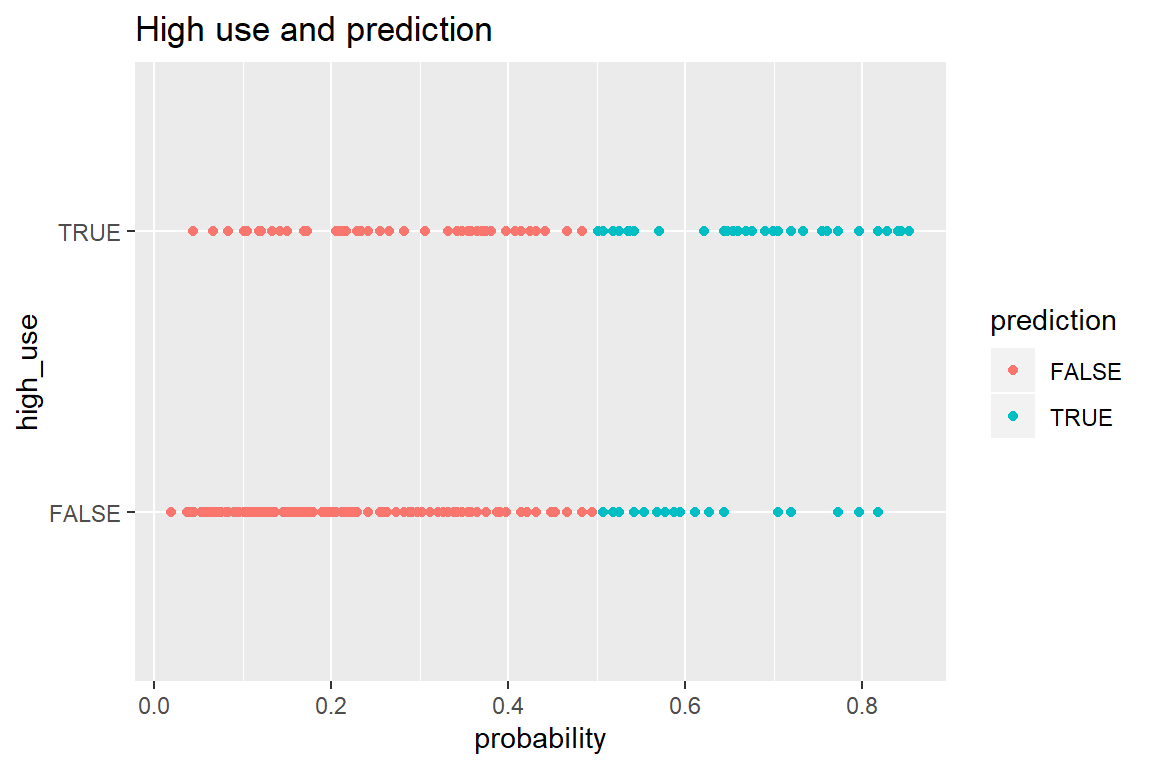
\includegraphics{index_files/figure-latex/unnamed-chunk-16-1.pdf}

Plotting reveals the same result. Most False high users are rightly
predicted as False high users, but most of those whose high\_us is true
are not predicted as true high users, although they should be. This
implies that the model doesn't work the way it should.

\begin{Shaded}
\begin{Highlighting}[]
\NormalTok{loss_func <-}\StringTok{ }\ControlFlowTok{function}\NormalTok{(class, prob) \{}
\NormalTok{  n_wrong <-}\StringTok{ }\KeywordTok{abs}\NormalTok{(class }\OperatorTok{-}\StringTok{ }\NormalTok{prob) }\OperatorTok{>}\StringTok{ }\FloatTok{0.5}
  \KeywordTok{mean}\NormalTok{(n_wrong)}
\NormalTok{\}}

\KeywordTok{loss_func}\NormalTok{(}\DataTypeTok{class =}\NormalTok{ alc}\OperatorTok{$}\NormalTok{high_use, }\DataTypeTok{prob =}\NormalTok{ alc}\OperatorTok{$}\NormalTok{probability)}
\end{Highlighting}
\end{Shaded}

\begin{verbatim}
## [1] 0.2303665
\end{verbatim}

The error is 0.230, which means 23\% percent of the predictions went
wrong.

If we compare this with simple guessing strategy (is someone high user
or not), where 1/2 so 50\% would go wrong, this model seems to be at
least better than just guessing.

\subsection{7) Bonus: 10-fold
cross-validation}\label{bonus-10-fold-cross-validation}

\begin{Shaded}
\begin{Highlighting}[]
\KeywordTok{library}\NormalTok{(boot)}
\NormalTok{cv <-}\StringTok{ }\KeywordTok{cv.glm}\NormalTok{(}\DataTypeTok{data =}\NormalTok{ alc, }\DataTypeTok{cost =}\NormalTok{ loss_func, }\DataTypeTok{glmfit =}\NormalTok{ m, }\DataTypeTok{K =} \DecValTok{10}\NormalTok{)}

\NormalTok{cv}\OperatorTok{$}\NormalTok{delta[}\DecValTok{1}\NormalTok{]}
\end{Highlighting}
\end{Shaded}

\begin{verbatim}
## [1] 0.2408377
\end{verbatim}

I got prediction errors between 0.23-0.25, so an error is bit higher
with the testing data compared to the training data. My model has a bit
smaller error than the one presented in Datacamp exercise.

\begin{center}\rule{0.5\linewidth}{\linethickness}\end{center}

\section{Week 4: Classification and
clustering}\label{week-4-classification-and-clustering}

\subsection{2) Getting to know dataset
Boston}\label{getting-to-know-dataset-boston}

\begin{verbatim}
## 'data.frame':    506 obs. of  14 variables:
##  $ crim   : num  0.00632 0.02731 0.02729 0.03237 0.06905 ...
##  $ zn     : num  18 0 0 0 0 0 12.5 12.5 12.5 12.5 ...
##  $ indus  : num  2.31 7.07 7.07 2.18 2.18 2.18 7.87 7.87 7.87 7.87 ...
##  $ chas   : int  0 0 0 0 0 0 0 0 0 0 ...
##  $ nox    : num  0.538 0.469 0.469 0.458 0.458 0.458 0.524 0.524 0.524 0.524 ...
##  $ rm     : num  6.58 6.42 7.18 7 7.15 ...
##  $ age    : num  65.2 78.9 61.1 45.8 54.2 58.7 66.6 96.1 100 85.9 ...
##  $ dis    : num  4.09 4.97 4.97 6.06 6.06 ...
##  $ rad    : int  1 2 2 3 3 3 5 5 5 5 ...
##  $ tax    : num  296 242 242 222 222 222 311 311 311 311 ...
##  $ ptratio: num  15.3 17.8 17.8 18.7 18.7 18.7 15.2 15.2 15.2 15.2 ...
##  $ black  : num  397 397 393 395 397 ...
##  $ lstat  : num  4.98 9.14 4.03 2.94 5.33 ...
##  $ medv   : num  24 21.6 34.7 33.4 36.2 28.7 22.9 27.1 16.5 18.9 ...
\end{verbatim}

This week we use Boston data set from R MASS package.

Boston has 14 variables and 506 observations.

As variables we have for example:\\
- per capita crime rate in town (crim)\\
- taxes (tax)\\
- socio-economic situation (lstat)\\
- distances (dis)\\
- infrastucture access (rad)\\
- nitrogen oxides concentration (nox)

More information:
\href{https://stat.ethz.ch/R-manual/R-devel/library/MASS/html/Boston.html}{link}

\subsection{3) Graphical overview and summaries of
variables}\label{graphical-overview-and-summaries-of-variables}

\begin{Shaded}
\begin{Highlighting}[]
\NormalTok{cor_matrix<-}\KeywordTok{cor}\NormalTok{(Boston) }

\KeywordTok{corrplot.mixed}\NormalTok{(cor_matrix, }\DataTypeTok{number.cex =}\NormalTok{ .}\DecValTok{6}\NormalTok{)}
\end{Highlighting}
\end{Shaded}

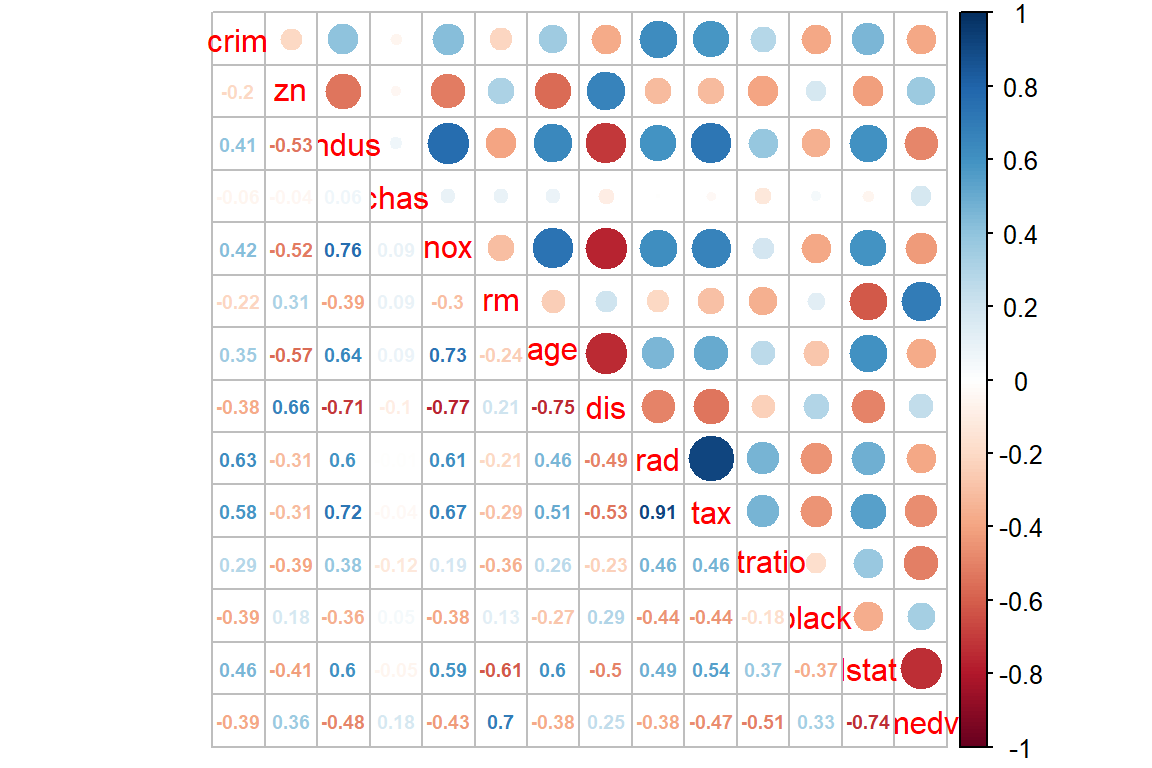
\includegraphics{index_files/figure-latex/unnamed-chunk-20-1.pdf}

\begin{Shaded}
\begin{Highlighting}[]
\KeywordTok{summary}\NormalTok{(Boston)}
\end{Highlighting}
\end{Shaded}

\begin{verbatim}
##       crim                zn             indus            chas        
##  Min.   : 0.00632   Min.   :  0.00   Min.   : 0.46   Min.   :0.00000  
##  1st Qu.: 0.08204   1st Qu.:  0.00   1st Qu.: 5.19   1st Qu.:0.00000  
##  Median : 0.25651   Median :  0.00   Median : 9.69   Median :0.00000  
##  Mean   : 3.61352   Mean   : 11.36   Mean   :11.14   Mean   :0.06917  
##  3rd Qu.: 3.67708   3rd Qu.: 12.50   3rd Qu.:18.10   3rd Qu.:0.00000  
##  Max.   :88.97620   Max.   :100.00   Max.   :27.74   Max.   :1.00000  
##       nox               rm             age              dis        
##  Min.   :0.3850   Min.   :3.561   Min.   :  2.90   Min.   : 1.130  
##  1st Qu.:0.4490   1st Qu.:5.886   1st Qu.: 45.02   1st Qu.: 2.100  
##  Median :0.5380   Median :6.208   Median : 77.50   Median : 3.207  
##  Mean   :0.5547   Mean   :6.285   Mean   : 68.57   Mean   : 3.795  
##  3rd Qu.:0.6240   3rd Qu.:6.623   3rd Qu.: 94.08   3rd Qu.: 5.188  
##  Max.   :0.8710   Max.   :8.780   Max.   :100.00   Max.   :12.127  
##       rad              tax           ptratio          black       
##  Min.   : 1.000   Min.   :187.0   Min.   :12.60   Min.   :  0.32  
##  1st Qu.: 4.000   1st Qu.:279.0   1st Qu.:17.40   1st Qu.:375.38  
##  Median : 5.000   Median :330.0   Median :19.05   Median :391.44  
##  Mean   : 9.549   Mean   :408.2   Mean   :18.46   Mean   :356.67  
##  3rd Qu.:24.000   3rd Qu.:666.0   3rd Qu.:20.20   3rd Qu.:396.23  
##  Max.   :24.000   Max.   :711.0   Max.   :22.00   Max.   :396.90  
##      lstat            medv      
##  Min.   : 1.73   Min.   : 5.00  
##  1st Qu.: 6.95   1st Qu.:17.02  
##  Median :11.36   Median :21.20  
##  Mean   :12.65   Mean   :22.53  
##  3rd Qu.:16.95   3rd Qu.:25.00  
##  Max.   :37.97   Max.   :50.00
\end{verbatim}

Corrplot shows the relationships between variables. Highest positive
correlations are between rad and tax, indus and nox and age and nox.
Highest negative correlations are between age and dis, lstat and med and
dis and nox.

When we look at the summaries of variables, we see that their
distributions are very different from eachother. This is why next we
need to scale them, so we can do linear discriminant analysis later.

\subsection{4) Scaling dataset and wrangling crime
variable}\label{scaling-dataset-and-wrangling-crime-variable}

\begin{Shaded}
\begin{Highlighting}[]
\NormalTok{boston_scaled <-}\StringTok{ }\KeywordTok{scale}\NormalTok{(Boston)}

\KeywordTok{summary}\NormalTok{(boston_scaled)}
\end{Highlighting}
\end{Shaded}

\begin{verbatim}
##       crim                 zn               indus        
##  Min.   :-0.419367   Min.   :-0.48724   Min.   :-1.5563  
##  1st Qu.:-0.410563   1st Qu.:-0.48724   1st Qu.:-0.8668  
##  Median :-0.390280   Median :-0.48724   Median :-0.2109  
##  Mean   : 0.000000   Mean   : 0.00000   Mean   : 0.0000  
##  3rd Qu.: 0.007389   3rd Qu.: 0.04872   3rd Qu.: 1.0150  
##  Max.   : 9.924110   Max.   : 3.80047   Max.   : 2.4202  
##       chas              nox                rm               age         
##  Min.   :-0.2723   Min.   :-1.4644   Min.   :-3.8764   Min.   :-2.3331  
##  1st Qu.:-0.2723   1st Qu.:-0.9121   1st Qu.:-0.5681   1st Qu.:-0.8366  
##  Median :-0.2723   Median :-0.1441   Median :-0.1084   Median : 0.3171  
##  Mean   : 0.0000   Mean   : 0.0000   Mean   : 0.0000   Mean   : 0.0000  
##  3rd Qu.:-0.2723   3rd Qu.: 0.5981   3rd Qu.: 0.4823   3rd Qu.: 0.9059  
##  Max.   : 3.6648   Max.   : 2.7296   Max.   : 3.5515   Max.   : 1.1164  
##       dis               rad               tax             ptratio       
##  Min.   :-1.2658   Min.   :-0.9819   Min.   :-1.3127   Min.   :-2.7047  
##  1st Qu.:-0.8049   1st Qu.:-0.6373   1st Qu.:-0.7668   1st Qu.:-0.4876  
##  Median :-0.2790   Median :-0.5225   Median :-0.4642   Median : 0.2746  
##  Mean   : 0.0000   Mean   : 0.0000   Mean   : 0.0000   Mean   : 0.0000  
##  3rd Qu.: 0.6617   3rd Qu.: 1.6596   3rd Qu.: 1.5294   3rd Qu.: 0.8058  
##  Max.   : 3.9566   Max.   : 1.6596   Max.   : 1.7964   Max.   : 1.6372  
##      black             lstat              medv        
##  Min.   :-3.9033   Min.   :-1.5296   Min.   :-1.9063  
##  1st Qu.: 0.2049   1st Qu.:-0.7986   1st Qu.:-0.5989  
##  Median : 0.3808   Median :-0.1811   Median :-0.1449  
##  Mean   : 0.0000   Mean   : 0.0000   Mean   : 0.0000  
##  3rd Qu.: 0.4332   3rd Qu.: 0.6024   3rd Qu.: 0.2683  
##  Max.   : 0.4406   Max.   : 3.5453   Max.   : 2.9865
\end{verbatim}

Scaling data makes variables comparable, when every mean is now zero.

\begin{Shaded}
\begin{Highlighting}[]
\CommentTok{# some more data wrangle for variable crime }

\NormalTok{boston_scaled <-}\StringTok{ }\KeywordTok{as.data.frame}\NormalTok{(boston_scaled)}

\NormalTok{bins <-}\StringTok{ }\KeywordTok{quantile}\NormalTok{(boston_scaled}\OperatorTok{$}\NormalTok{crim)}

\NormalTok{crime <-}\StringTok{ }\KeywordTok{cut}\NormalTok{(boston_scaled}\OperatorTok{$}\NormalTok{crim, }\DataTypeTok{breaks =}\NormalTok{ bins, }\DataTypeTok{include.lowest =} \OtherTok{TRUE}\NormalTok{, }\DataTypeTok{label =} \KeywordTok{c}\NormalTok{(}\StringTok{"low"}\NormalTok{, }\StringTok{"med_low"}\NormalTok{, }\StringTok{"med_high"}\NormalTok{, }\StringTok{"high"}\NormalTok{))}

\NormalTok{boston_scaled <-}\StringTok{ }\NormalTok{dplyr}\OperatorTok{::}\KeywordTok{select}\NormalTok{(boston_scaled, }\OperatorTok{-}\NormalTok{crim)}

\NormalTok{boston_scaled <-}\StringTok{ }\KeywordTok{data.frame}\NormalTok{(boston_scaled, crime)}

\CommentTok{# creating train and test datasets}

\NormalTok{n <-}\StringTok{ }\KeywordTok{nrow}\NormalTok{(boston_scaled)}

\NormalTok{rows <-}\StringTok{ }\KeywordTok{sample}\NormalTok{(n, }\DataTypeTok{size =}\NormalTok{ n}\OperatorTok{*}\FloatTok{0.8}\NormalTok{)}

\NormalTok{train <-}\StringTok{ }\NormalTok{boston_scaled[rows,]}

\NormalTok{test <-}\StringTok{ }\NormalTok{boston_scaled[}\OperatorTok{-}\NormalTok{rows,]}
\end{Highlighting}
\end{Shaded}

\subsection{5) Fitting linear discriminant
analysis}\label{fitting-linear-discriminant-analysis}

\begin{Shaded}
\begin{Highlighting}[]
\NormalTok{lda.m <-}\StringTok{ }\KeywordTok{lda}\NormalTok{(crime }\OperatorTok{~}\StringTok{ }\NormalTok{., }\DataTypeTok{data =}\NormalTok{ train)}
\NormalTok{lda.m}
\end{Highlighting}
\end{Shaded}

\begin{verbatim}
## Call:
## lda(crime ~ ., data = train)
## 
## Prior probabilities of groups:
##       low   med_low  med_high      high 
## 0.2450495 0.2400990 0.2475248 0.2673267 
## 
## Group means:
##                  zn      indus        chas        nox         rm
## low       0.9346350 -0.9247560 -0.15302300 -0.8817214  0.4944457
## med_low  -0.1039982 -0.2426125 -0.06938576 -0.5731711 -0.1233464
## med_high -0.3997708  0.2009403  0.16075196  0.4336033  0.0118352
## high     -0.4872402  1.0169921 -0.01714665  1.0545071 -0.4341640
##                 age        dis        rad        tax    ptratio
## low      -0.9298742  0.9422660 -0.6941744 -0.7379892 -0.4348341
## med_low  -0.3181779  0.3228979 -0.5662919 -0.4544261 -0.0561275
## med_high  0.3903213 -0.3533652 -0.4283101 -0.3125552 -0.2806230
## high      0.8137658 -0.8607469  1.6393984  1.5149640  0.7822555
##                black       lstat          medv
## low       0.37287115 -0.77510653  0.5658919768
## med_low   0.33918067 -0.15970818 -0.0003163405
## med_high  0.06048827  0.02404919  0.1191890040
## high     -0.72356464  0.86781523 -0.6482949303
## 
## Coefficients of linear discriminants:
##                  LD1         LD2         LD3
## zn       0.113306958  0.68296468 -0.72856501
## indus    0.014203528 -0.20169087  0.42273178
## chas    -0.014130026 -0.05198378  0.11873941
## nox      0.367526306 -0.57780808 -1.60024923
## rm       0.005989688  0.05024122 -0.19658478
## age      0.202366242 -0.37210058  0.02590554
## dis     -0.130520302 -0.14127996 -0.06500505
## rad      3.398974329  0.85297961 -0.05768677
## tax     -0.023874669  0.03834024  0.54987113
## ptratio  0.144024531  0.05621746 -0.30255953
## black   -0.111146301  0.04165159  0.18487866
## lstat    0.183159234 -0.17019429  0.22402631
## medv     0.071747708 -0.30870174 -0.28686793
## 
## Proportion of trace:
##    LD1    LD2    LD3 
## 0.9564 0.0322 0.0114
\end{verbatim}

\begin{Shaded}
\begin{Highlighting}[]
\CommentTok{# and plotting}
\CommentTok{# arrows}

\NormalTok{lda.arrows <-}\StringTok{ }\ControlFlowTok{function}\NormalTok{(x, }\DataTypeTok{myscale =} \DecValTok{1}\NormalTok{, }\DataTypeTok{arrow_heads =} \FloatTok{0.1}\NormalTok{, }\DataTypeTok{color =} \StringTok{"red"}\NormalTok{, }\DataTypeTok{tex =} \FloatTok{0.75}\NormalTok{, }\DataTypeTok{choices =} \KeywordTok{c}\NormalTok{(}\DecValTok{1}\NormalTok{,}\DecValTok{2}\NormalTok{))\{}
\NormalTok{  heads <-}\StringTok{ }\KeywordTok{coef}\NormalTok{(x)}
  \KeywordTok{arrows}\NormalTok{(}\DataTypeTok{x0 =} \DecValTok{0}\NormalTok{, }\DataTypeTok{y0 =} \DecValTok{0}\NormalTok{, }
         \DataTypeTok{x1 =}\NormalTok{ myscale }\OperatorTok{*}\StringTok{ }\NormalTok{heads[,choices[}\DecValTok{1}\NormalTok{]], }
         \DataTypeTok{y1 =}\NormalTok{ myscale }\OperatorTok{*}\StringTok{ }\NormalTok{heads[,choices[}\DecValTok{2}\NormalTok{]], }\DataTypeTok{col=}\NormalTok{color, }\DataTypeTok{length =}\NormalTok{ arrow_heads)}
  \KeywordTok{text}\NormalTok{(myscale }\OperatorTok{*}\StringTok{ }\NormalTok{heads[,choices], }\DataTypeTok{labels =} \KeywordTok{row.names}\NormalTok{(heads), }
       \DataTypeTok{cex =}\NormalTok{ tex, }\DataTypeTok{col=}\NormalTok{color, }\DataTypeTok{pos=}\DecValTok{3}\NormalTok{)}
\NormalTok{\}}

\NormalTok{classes <-}\StringTok{ }\KeywordTok{as.numeric}\NormalTok{(train}\OperatorTok{$}\NormalTok{crime)}

\KeywordTok{plot}\NormalTok{(lda.m, }\DataTypeTok{dimen =} \DecValTok{2}\NormalTok{, }\DataTypeTok{col =}\NormalTok{ classes, }\DataTypeTok{pch =}\NormalTok{ classes)}
\KeywordTok{lda.arrows}\NormalTok{(lda.m, }\DataTypeTok{myscale =} \DecValTok{2}\NormalTok{)}
\end{Highlighting}
\end{Shaded}

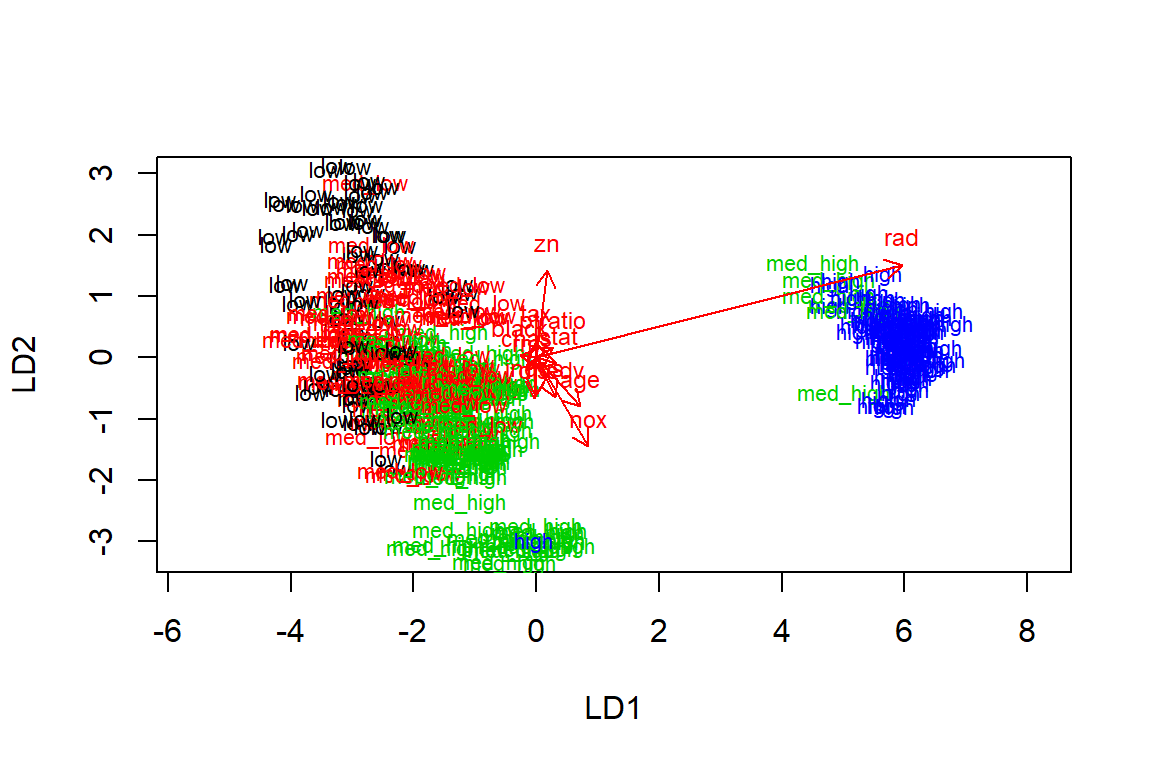
\includegraphics{index_files/figure-latex/unnamed-chunk-23-1.pdf}

Most clear class seems to be high crime rate. Med\_high and med\_low
classes seem to blend within eachother and low class is also really
spread. The variables with biggest effects (longest arrows) are rad, zn
and nox.

\subsection{6) Prediction based on the fitted
model}\label{prediction-based-on-the-fitted-model}

\begin{Shaded}
\begin{Highlighting}[]
\NormalTok{correct_classes <-}\StringTok{ }\NormalTok{test}\OperatorTok{$}\NormalTok{crime}

\NormalTok{test <-}\StringTok{ }\NormalTok{dplyr}\OperatorTok{::}\KeywordTok{select}\NormalTok{(test, }\OperatorTok{-}\NormalTok{crime)}

\NormalTok{lda.pre <-}\StringTok{ }\KeywordTok{predict}\NormalTok{(lda.m, }\DataTypeTok{newdata =}\NormalTok{ test)}

\KeywordTok{table}\NormalTok{(}\DataTypeTok{correct =}\NormalTok{ correct_classes, }\DataTypeTok{predictions =}\NormalTok{ lda.pre}\OperatorTok{$}\NormalTok{class)}
\end{Highlighting}
\end{Shaded}

\begin{verbatim}
##           predictions
## correct    low med_low med_high high
##   low       15      13        0    0
##   med_low    7      19        3    0
##   med_high   0       6       18    2
##   high       0       0        0   19
\end{verbatim}

The cross table shows that high values were predicted correctly. In
other classes there are more errors, which was also implied from the
plot above. This means that training data didnt succeed that well with
our model, or that maybe we should think about defining the classes
again.

\subsection{7) Clustering}\label{clustering}

\begin{Shaded}
\begin{Highlighting}[]
\CommentTok{# Lets read the data again and scale it}

\KeywordTok{data}\NormalTok{(}\StringTok{"Boston"}\NormalTok{)}

\NormalTok{c_boston_scaled <-}\StringTok{ }\KeywordTok{scale}\NormalTok{(Boston)}

\CommentTok{# Distances with euclidean distance}
\NormalTok{dist_eu <-}\StringTok{ }\KeywordTok{dist}\NormalTok{(c_boston_scaled)}

\KeywordTok{summary}\NormalTok{(dist_eu)}
\end{Highlighting}
\end{Shaded}

\begin{verbatim}
##    Min. 1st Qu.  Median    Mean 3rd Qu.    Max. 
##  0.1343  3.4625  4.8241  4.9111  6.1863 14.3970
\end{verbatim}

\begin{Shaded}
\begin{Highlighting}[]
\NormalTok{km <-}\StringTok{ }\KeywordTok{kmeans}\NormalTok{(c_boston_scaled, }\DataTypeTok{centers =} \DecValTok{3}\NormalTok{)}

\KeywordTok{set.seed}\NormalTok{(}\DecValTok{123}\NormalTok{)}
\NormalTok{k_max <-}\StringTok{ }\DecValTok{10}
\NormalTok{twcss <-}\StringTok{ }\KeywordTok{sapply}\NormalTok{(}\DecValTok{1}\OperatorTok{:}\NormalTok{k_max, }\ControlFlowTok{function}\NormalTok{(k)\{}\KeywordTok{kmeans}\NormalTok{(c_boston_scaled, k)}\OperatorTok{$}\NormalTok{tot.withinss\})}
\KeywordTok{qplot}\NormalTok{(}\DataTypeTok{x =} \DecValTok{1}\OperatorTok{:}\NormalTok{k_max, }\DataTypeTok{y =}\NormalTok{ twcss, }\DataTypeTok{geom =} \StringTok{'line'}\NormalTok{)}
\end{Highlighting}
\end{Shaded}

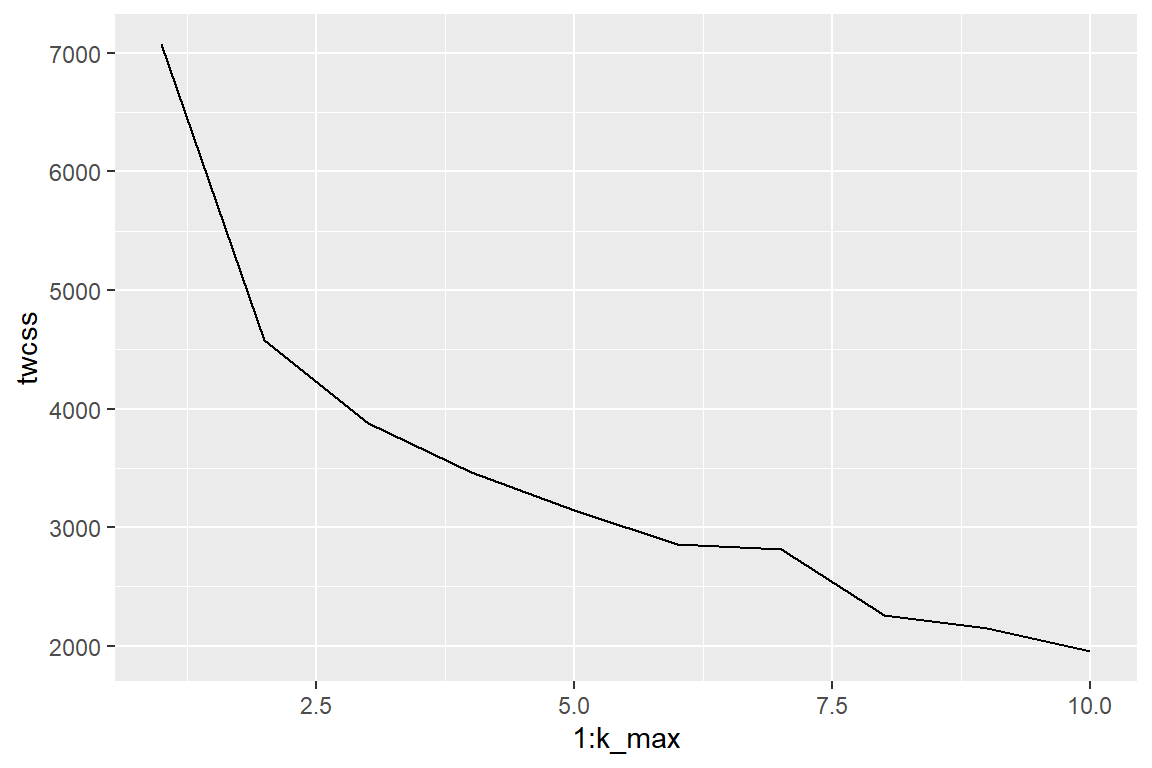
\includegraphics{index_files/figure-latex/unnamed-chunk-26-1.pdf}

The optimal cluster size is the point where the line drops radically.
This seems to be two.

\begin{Shaded}
\begin{Highlighting}[]
\CommentTok{# Clustering with two}

\NormalTok{km2 <-}\StringTok{ }\KeywordTok{kmeans}\NormalTok{(c_boston_scaled, }\DataTypeTok{centers =} \DecValTok{2}\NormalTok{)}

\KeywordTok{pairs}\NormalTok{(c_boston_scaled[,}\DecValTok{1}\OperatorTok{:}\DecValTok{7}\NormalTok{], }\DataTypeTok{col =}\NormalTok{ km2}\OperatorTok{$}\NormalTok{cluster)}
\end{Highlighting}
\end{Shaded}

\includegraphics{index_files/figure-latex/unnamed-chunk-27-1.pdf}

\begin{Shaded}
\begin{Highlighting}[]
\KeywordTok{pairs}\NormalTok{(c_boston_scaled[,}\DecValTok{8}\OperatorTok{:}\DecValTok{14}\NormalTok{], }\DataTypeTok{col =}\NormalTok{ km2}\OperatorTok{$}\NormalTok{cluster)}
\end{Highlighting}
\end{Shaded}

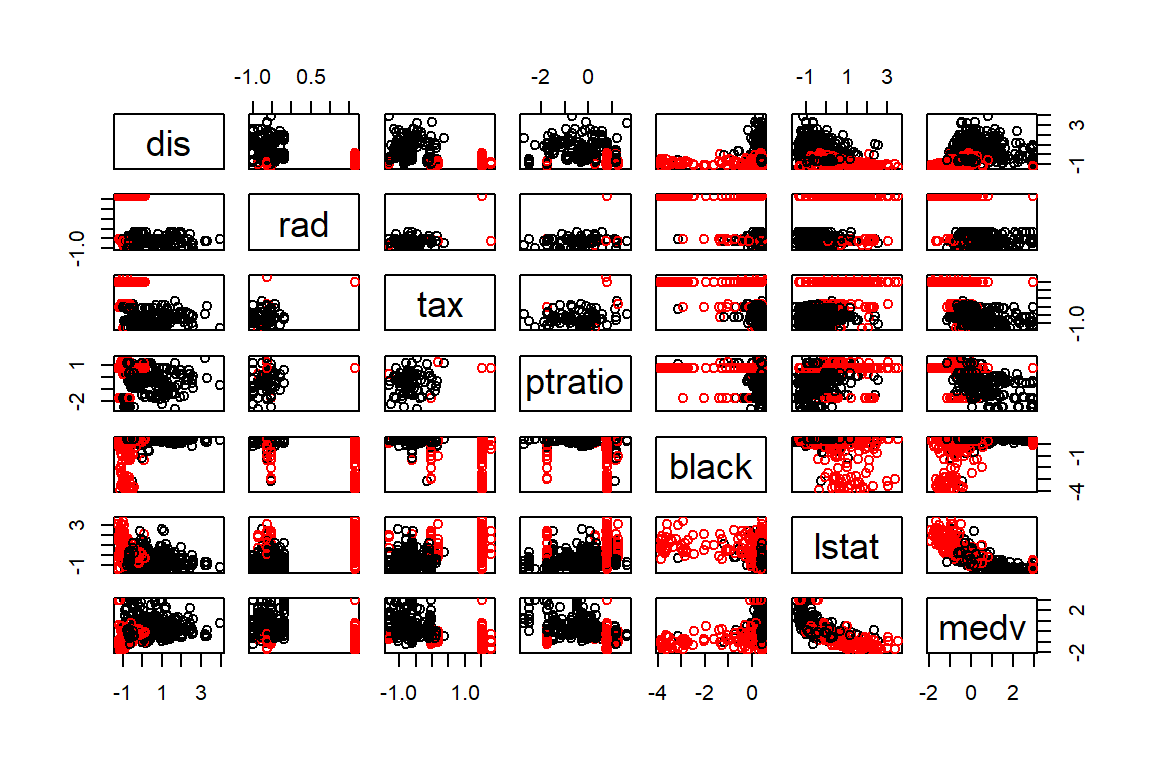
\includegraphics{index_files/figure-latex/unnamed-chunk-27-2.pdf}

So now we have found out, that this dataset could be divided to two
clusters.

In the pairs plots we see, that between some variables the clustering
works better than with some. Clusters are well seen for example within
nox and rm and then not so clear between rad and tax.

\begin{center}\rule{0.5\linewidth}{\linethickness}\end{center}

\section{Week 5: Dimensionality reduction
techniques}\label{week-5-dimensionality-reduction-techniques}

This week I'll dive into dimensionality reduction techniques.

\subsection{1) Graphical overview and summaries of the
data}\label{graphical-overview-and-summaries-of-the-data}

\begin{Shaded}
\begin{Highlighting}[]
\KeywordTok{library}\NormalTok{(MASS); }\KeywordTok{library}\NormalTok{(dplyr); }\KeywordTok{library}\NormalTok{(ggplot2); }\KeywordTok{library}\NormalTok{(GGally); }\KeywordTok{library}\NormalTok{(tidyr)}

\NormalTok{human <-}\StringTok{ }\KeywordTok{read.csv2}\NormalTok{(}\DataTypeTok{file =} \StringTok{"data/human.csv"}\NormalTok{, }\DataTypeTok{sep =} \StringTok{","}\NormalTok{, }\DataTypeTok{dec =} \StringTok{"."}\NormalTok{)}

\KeywordTok{str}\NormalTok{(human)}
\end{Highlighting}
\end{Shaded}

\begin{verbatim}
## 'data.frame':    155 obs. of  8 variables:
##  $ Edu2.FM  : num  1.007 0.997 0.983 0.989 0.969 ...
##  $ Labo.FM  : num  0.891 0.819 0.825 0.884 0.829 ...
##  $ Edu.Exp  : num  17.5 20.2 15.8 18.7 17.9 16.5 18.6 16.5 15.9 19.2 ...
##  $ Life.Exp : num  81.6 82.4 83 80.2 81.6 80.9 80.9 79.1 82 81.8 ...
##  $ GNI      : int  166 135 156 139 140 137 127 154 134 117 ...
##  $ Mat.Mor  : int  4 6 6 5 6 7 9 28 11 8 ...
##  $ Ado.Birth: num  7.8 12.1 1.9 5.1 6.2 3.8 8.2 31 14.5 25.3 ...
##  $ Parli.F  : num  39.6 30.5 28.5 38 36.9 36.9 19.9 19.4 28.2 31.4 ...
\end{verbatim}

\begin{Shaded}
\begin{Highlighting}[]
\NormalTok{g1 <-}\StringTok{ }\KeywordTok{ggpairs}\NormalTok{(human)}
\NormalTok{g1}
\end{Highlighting}
\end{Shaded}

\includegraphics{index_files/figure-latex/unnamed-chunk-28-1.pdf}

\begin{Shaded}
\begin{Highlighting}[]
\KeywordTok{summary}\NormalTok{(human)}
\end{Highlighting}
\end{Shaded}

\begin{verbatim}
##     Edu2.FM          Labo.FM          Edu.Exp         Life.Exp    
##  Min.   :0.1717   Min.   :0.1857   Min.   : 5.40   Min.   :49.00  
##  1st Qu.:0.7264   1st Qu.:0.5984   1st Qu.:11.25   1st Qu.:66.30  
##  Median :0.9375   Median :0.7535   Median :13.50   Median :74.20  
##  Mean   :0.8529   Mean   :0.7074   Mean   :13.18   Mean   :71.65  
##  3rd Qu.:0.9968   3rd Qu.:0.8535   3rd Qu.:15.20   3rd Qu.:77.25  
##  Max.   :1.4967   Max.   :1.0380   Max.   :20.20   Max.   :83.50  
##       GNI            Mat.Mor         Ado.Birth         Parli.F     
##  Min.   :  2.00   Min.   :   1.0   Min.   :  0.60   Min.   : 0.00  
##  1st Qu.: 53.50   1st Qu.:  11.5   1st Qu.: 12.65   1st Qu.:12.40  
##  Median : 99.00   Median :  49.0   Median : 33.60   Median :19.30  
##  Mean   : 98.73   Mean   : 149.1   Mean   : 47.16   Mean   :20.91  
##  3rd Qu.:143.50   3rd Qu.: 190.0   3rd Qu.: 71.95   3rd Qu.:27.95  
##  Max.   :194.00   Max.   :1100.0   Max.   :204.80   Max.   :57.50
\end{verbatim}

Data has 8 variables and 155 observations, which are countries.

From the pairs plot we see that Life.exp and Edu.exp and Mat.Mor and
Ado.Birth have a high positive correlation. Life.exp has a high negative
correlation both with Mat.mor \& Ado.birth.

From summaries we see that for example there is a high variation in
life.exp and edu.exp between observations.

\subsection{2) Principal component analysis (PCA) not
standardised}\label{principal-component-analysis-pca-not-standardised}

\begin{Shaded}
\begin{Highlighting}[]
\CommentTok{# perform principal component analysis (with the SVD method)}
\NormalTok{pca_human <-}\StringTok{ }\KeywordTok{prcomp}\NormalTok{(human)}

\KeywordTok{summary}\NormalTok{(pca_human)}
\end{Highlighting}
\end{Shaded}

\begin{verbatim}
## Importance of components:
##                             PC1      PC2      PC3      PC4     PC5     PC6
## Standard deviation     214.3202 54.48589 26.38141 11.47911 4.06687 1.60671
## Proportion of Variance   0.9233  0.05967  0.01399  0.00265 0.00033 0.00005
## Cumulative Proportion    0.9233  0.98298  0.99697  0.99961 0.99995 1.00000
##                           PC7    PC8
## Standard deviation     0.1905 0.1587
## Proportion of Variance 0.0000 0.0000
## Cumulative Proportion  1.0000 1.0000
\end{verbatim}

\begin{Shaded}
\begin{Highlighting}[]
\CommentTok{# draw a biplot of the principal component representation and the original variables}
\KeywordTok{biplot}\NormalTok{(pca_human, }\DataTypeTok{choices =} \DecValTok{1}\OperatorTok{:}\DecValTok{2}\NormalTok{, }\DataTypeTok{cex =} \KeywordTok{c}\NormalTok{(}\FloatTok{0.7}\NormalTok{,}\DecValTok{1}\NormalTok{), }\DataTypeTok{col =} \KeywordTok{c}\NormalTok{(}\StringTok{"grey40"}\NormalTok{, }\StringTok{"deeppink2"}\NormalTok{), }\DataTypeTok{xlab =} \StringTok{"PC1: Maternity mortality"}\NormalTok{, }\DataTypeTok{ylab =} \StringTok{"PC2: GNI"}\NormalTok{)}
\end{Highlighting}
\end{Shaded}

\begin{verbatim}
## Warning in arrows(0, 0, y[, 1L] * 0.8, y[, 2L] * 0.8, col = col[2L], length
## = arrow.len): zero-length arrow is of indeterminate angle and so skipped
\end{verbatim}

\includegraphics{index_files/figure-latex/unnamed-chunk-29-1.pdf}

\subsection{3) Same but standardized}\label{same-but-standardized}

\begin{Shaded}
\begin{Highlighting}[]
\NormalTok{human_std <-}\StringTok{ }\KeywordTok{scale}\NormalTok{(human)}

\CommentTok{# perform principal component analysis (with the SVD method)}
\NormalTok{pca_human_std <-}\StringTok{ }\KeywordTok{prcomp}\NormalTok{(human_std)}

\KeywordTok{summary}\NormalTok{(pca_human_std)}
\end{Highlighting}
\end{Shaded}

\begin{verbatim}
## Importance of components:
##                          PC1    PC2    PC3     PC4     PC5     PC6     PC7
## Standard deviation     1.966 1.1388 0.9900 0.86598 0.69931 0.54001 0.46701
## Proportion of Variance 0.483 0.1621 0.1225 0.09374 0.06113 0.03645 0.02726
## Cumulative Proportion  0.483 0.6452 0.7677 0.86140 0.92253 0.95898 0.98625
##                            PC8
## Standard deviation     0.33172
## Proportion of Variance 0.01375
## Cumulative Proportion  1.00000
\end{verbatim}

\begin{Shaded}
\begin{Highlighting}[]
\CommentTok{# draw a biplot of the principal component representation and the original variables}
\KeywordTok{biplot}\NormalTok{(pca_human_std, }\DataTypeTok{choices =} \DecValTok{1}\OperatorTok{:}\DecValTok{2}\NormalTok{, }\DataTypeTok{cex =} \KeywordTok{c}\NormalTok{(}\FloatTok{0.8}\NormalTok{,}\DecValTok{1}\NormalTok{), }\DataTypeTok{col =} \KeywordTok{c}\NormalTok{(}\StringTok{"grey40"}\NormalTok{, }\StringTok{"deeppink2"}\NormalTok{), }\DataTypeTok{xlab=}\StringTok{"PC1: Health and education"}\NormalTok{, }\DataTypeTok{ylab=}\StringTok{"PC2: Women in work and public life"}\NormalTok{)}
\end{Highlighting}
\end{Shaded}

\includegraphics{index_files/figure-latex/unnamed-chunk-30-1.pdf}

Results of the standardized and non-standardized PCA are very different,
since on the non standardized version the variabels with very high
values get more weight in the analysis.

The non-standarized PC1 has Mat.Mor as a contributor, and PC2 GNI as a
contributor. Both of them have really high standard deviations 214.3 and
54.5, which is caused by the missing scaling and high deviation of
Mat.Mor and GNI.

Then on the scaled PC1 and PC2 the sd:s are 1.966 and 1.1388, which is a
lot better. Therefor scaled Principal components have more contributing
variables, when Mat.mor and GNI are not overweighting anymore.

\subsection{4) Personal interpretation on the standardized PC1 ans
PC2}\label{personal-interpretation-on-the-standardized-pc1-ans-pc2}

Mat.Mor, Ado.Birth, Edu.Exp, Edu2.FM, GNI and Life.Exp are pointing on
PC1 axis, so they contribute to Principal component 1. This means that
PC1 consist about Health related variables (life expectency, maternity
mortality) and education (ratio and expected time).

Parli.F and Labo.FM are pointing towards PC2 axis, which mean they
contribute to Principal component 2. This means PC2 consist of womens
repsentation in the work and official public life.

\subsection{5) Multiple Correspondence
Analysis}\label{multiple-correspondence-analysis}

\begin{Shaded}
\begin{Highlighting}[]
\KeywordTok{library}\NormalTok{(FactoMineR)}

\KeywordTok{data}\NormalTok{(}\StringTok{"tea"}\NormalTok{)}

\KeywordTok{str}\NormalTok{(tea)}
\end{Highlighting}
\end{Shaded}

\begin{verbatim}
## 'data.frame':    300 obs. of  36 variables:
##  $ breakfast       : Factor w/ 2 levels "breakfast","Not.breakfast": 1 1 2 2 1 2 1 2 1 1 ...
##  $ tea.time        : Factor w/ 2 levels "Not.tea time",..: 1 1 2 1 1 1 2 2 2 1 ...
##  $ evening         : Factor w/ 2 levels "evening","Not.evening": 2 2 1 2 1 2 2 1 2 1 ...
##  $ lunch           : Factor w/ 2 levels "lunch","Not.lunch": 2 2 2 2 2 2 2 2 2 2 ...
##  $ dinner          : Factor w/ 2 levels "dinner","Not.dinner": 2 2 1 1 2 1 2 2 2 2 ...
##  $ always          : Factor w/ 2 levels "always","Not.always": 2 2 2 2 1 2 2 2 2 2 ...
##  $ home            : Factor w/ 2 levels "home","Not.home": 1 1 1 1 1 1 1 1 1 1 ...
##  $ work            : Factor w/ 2 levels "Not.work","work": 1 1 2 1 1 1 1 1 1 1 ...
##  $ tearoom         : Factor w/ 2 levels "Not.tearoom",..: 1 1 1 1 1 1 1 1 1 2 ...
##  $ friends         : Factor w/ 2 levels "friends","Not.friends": 2 2 1 2 2 2 1 2 2 2 ...
##  $ resto           : Factor w/ 2 levels "Not.resto","resto": 1 1 2 1 1 1 1 1 1 1 ...
##  $ pub             : Factor w/ 2 levels "Not.pub","pub": 1 1 1 1 1 1 1 1 1 1 ...
##  $ Tea             : Factor w/ 3 levels "black","Earl Grey",..: 1 1 2 2 2 2 2 1 2 1 ...
##  $ How             : Factor w/ 4 levels "alone","lemon",..: 1 3 1 1 1 1 1 3 3 1 ...
##  $ sugar           : Factor w/ 2 levels "No.sugar","sugar": 2 1 1 2 1 1 1 1 1 1 ...
##  $ how             : Factor w/ 3 levels "tea bag","tea bag+unpackaged",..: 1 1 1 1 1 1 1 1 2 2 ...
##  $ where           : Factor w/ 3 levels "chain store",..: 1 1 1 1 1 1 1 1 2 2 ...
##  $ price           : Factor w/ 6 levels "p_branded","p_cheap",..: 4 6 6 6 6 3 6 6 5 5 ...
##  $ age             : int  39 45 47 23 48 21 37 36 40 37 ...
##  $ sex             : Factor w/ 2 levels "F","M": 2 1 1 2 2 2 2 1 2 2 ...
##  $ SPC             : Factor w/ 7 levels "employee","middle",..: 2 2 4 6 1 6 5 2 5 5 ...
##  $ Sport           : Factor w/ 2 levels "Not.sportsman",..: 2 2 2 1 2 2 2 2 2 1 ...
##  $ age_Q           : Factor w/ 5 levels "15-24","25-34",..: 3 4 4 1 4 1 3 3 3 3 ...
##  $ frequency       : Factor w/ 4 levels "1/day","1 to 2/week",..: 1 1 3 1 3 1 4 2 3 3 ...
##  $ escape.exoticism: Factor w/ 2 levels "escape-exoticism",..: 2 1 2 1 1 2 2 2 2 2 ...
##  $ spirituality    : Factor w/ 2 levels "Not.spirituality",..: 1 1 1 2 2 1 1 1 1 1 ...
##  $ healthy         : Factor w/ 2 levels "healthy","Not.healthy": 1 1 1 1 2 1 1 1 2 1 ...
##  $ diuretic        : Factor w/ 2 levels "diuretic","Not.diuretic": 2 1 1 2 1 2 2 2 2 1 ...
##  $ friendliness    : Factor w/ 2 levels "friendliness",..: 2 2 1 2 1 2 2 1 2 1 ...
##  $ iron.absorption : Factor w/ 2 levels "iron absorption",..: 2 2 2 2 2 2 2 2 2 2 ...
##  $ feminine        : Factor w/ 2 levels "feminine","Not.feminine": 2 2 2 2 2 2 2 1 2 2 ...
##  $ sophisticated   : Factor w/ 2 levels "Not.sophisticated",..: 1 1 1 2 1 1 1 2 2 1 ...
##  $ slimming        : Factor w/ 2 levels "No.slimming",..: 1 1 1 1 1 1 1 1 1 1 ...
##  $ exciting        : Factor w/ 2 levels "exciting","No.exciting": 2 1 2 2 2 2 2 2 2 2 ...
##  $ relaxing        : Factor w/ 2 levels "No.relaxing",..: 1 1 2 2 2 2 2 2 2 2 ...
##  $ effect.on.health: Factor w/ 2 levels "effect on health",..: 2 2 2 2 2 2 2 2 2 2 ...
\end{verbatim}

\begin{Shaded}
\begin{Highlighting}[]
\CommentTok{# visualizing variables home, work, tearoom, friends, resto, pub, Tea, How, sugar}
\KeywordTok{gather}\NormalTok{(tea[,}\DecValTok{7}\OperatorTok{:}\DecValTok{15}\NormalTok{]) }\OperatorTok\StringTok{ }\KeywordTok{ggplot}\NormalTok{(}\KeywordTok{aes}\NormalTok{(value)) }\OperatorTok{+}\StringTok{ }\KeywordTok{facet_wrap}\NormalTok{(}\StringTok{"key"}\NormalTok{, }\DataTypeTok{scales =} \StringTok{"free"}\NormalTok{) }\OperatorTok{+}\StringTok{ }\KeywordTok{geom_bar}\NormalTok{() }\OperatorTok{+}\StringTok{ }\KeywordTok{theme}\NormalTok{(}\DataTypeTok{axis.text.x =} \KeywordTok{element_text}\NormalTok{(}\DataTypeTok{angle =} \DecValTok{45}\NormalTok{, }\DataTypeTok{hjust =} \DecValTok{1}\NormalTok{, }\DataTypeTok{size =} \DecValTok{8}\NormalTok{))}
\end{Highlighting}
\end{Shaded}

\begin{verbatim}
## Warning: attributes are not identical across measure variables;
## they will be dropped
\end{verbatim}

\includegraphics{index_files/figure-latex/unnamed-chunk-31-1.pdf}

Tea is a dataset of different factor variables (36) connected to tea
drinking on 300 observations.

\begin{Shaded}
\begin{Highlighting}[]
\CommentTok{# MCA with variables: home, work, tearoom, friends, resto, pub, Tea, How, sugar}
\NormalTok{mca <-}\StringTok{ }\KeywordTok{MCA}\NormalTok{(tea[,}\DecValTok{7}\OperatorTok{:}\DecValTok{15}\NormalTok{], }\DataTypeTok{graph =} \OtherTok{FALSE}\NormalTok{)}

\CommentTok{# summary of the model}
\KeywordTok{summary}\NormalTok{(mca)}
\end{Highlighting}
\end{Shaded}

\begin{verbatim}
## 
## Call:
## MCA(X = tea[, 7:15], graph = FALSE) 
## 
## 
## Eigenvalues
##                        Dim.1   Dim.2   Dim.3   Dim.4   Dim.5   Dim.6
## Variance               0.206   0.161   0.126   0.121   0.114   0.107
## % of var.             15.415  12.043   9.433   9.108   8.585   8.031
## Cumulative % of var.  15.415  27.458  36.891  45.999  54.585  62.615
##                        Dim.7   Dim.8   Dim.9  Dim.10  Dim.11  Dim.12
## Variance               0.103   0.093   0.088   0.080   0.069   0.065
## % of var.              7.713   6.971   6.636   5.973   5.208   4.884
## Cumulative % of var.  70.328  77.299  83.935  89.908  95.116 100.000
## 
## Individuals (the 10 first)
##                Dim.1    ctr   cos2    Dim.2    ctr   cos2    Dim.3    ctr
## 1           | -0.512  0.424  0.300 |  0.208  0.090  0.049 |  0.180  0.086
## 2           | -0.474  0.364  0.185 |  0.621  0.802  0.318 |  0.581  0.894
## 3           |  0.392  0.249  0.165 | -0.038  0.003  0.002 |  0.002  0.000
## 4           | -0.461  0.345  0.358 | -0.264  0.144  0.117 |  0.086  0.020
## 5           | -0.472  0.361  0.384 |  0.052  0.006  0.005 | -0.111  0.032
## 6           | -0.472  0.361  0.384 |  0.052  0.006  0.005 | -0.111  0.032
## 7           | -0.200  0.065  0.094 | -0.036  0.003  0.003 | -0.276  0.201
## 8           | -0.474  0.364  0.185 |  0.621  0.802  0.318 |  0.581  0.894
## 9           | -0.423  0.291  0.191 |  0.150  0.047  0.024 |  0.487  0.627
## 10          | -0.170  0.047  0.022 |  0.714  1.059  0.394 | -0.151  0.060
##               cos2  
## 1            0.037 |
## 2            0.278 |
## 3            0.000 |
## 4            0.012 |
## 5            0.021 |
## 6            0.021 |
## 7            0.177 |
## 8            0.278 |
## 9            0.252 |
## 10           0.018 |
## 
## Categories (the 10 first)
##                 Dim.1     ctr    cos2  v.test     Dim.2     ctr    cos2
## home        |  -0.013   0.008   0.005  -1.240 |   0.063   0.270   0.130
## Not.home    |   0.408   0.270   0.005   1.240 |  -2.051   8.734   0.130
## Not.work    |  -0.278   2.971   0.189  -7.527 |   0.101   0.504   0.025
## work        |   0.681   7.273   0.189   7.527 |  -0.248   1.235   0.025
## Not.tearoom |  -0.278   3.370   0.322  -9.819 |  -0.133   0.986   0.074
## tearoom     |   1.160  14.063   0.322   9.819 |   0.554   4.112   0.074
## friends     |   0.384   5.203   0.278   9.111 |  -0.111   0.558   0.023
## Not.friends |  -0.723   9.805   0.278  -9.111 |   0.209   1.052   0.023
## Not.resto   |  -0.383   5.856   0.411 -11.091 |  -0.091   0.419   0.023
## resto       |   1.073  16.383   0.411  11.091 |   0.254   1.171   0.023
##              v.test     Dim.3     ctr    cos2  v.test  
## home          6.238 |  -0.018   0.027   0.010  -1.761 |
## Not.home     -6.238 |   0.579   0.889   0.010   1.761 |
## Not.work      2.741 |  -0.158   1.560   0.061  -4.267 |
## work         -2.741 |   0.386   3.819   0.061   4.267 |
## Not.tearoom  -4.693 |   0.083   0.489   0.029   2.926 |
## tearoom       4.693 |  -0.346   2.041   0.029  -2.926 |
## friends      -2.637 |  -0.182   1.921   0.063  -4.331 |
## Not.friends   2.637 |   0.344   3.620   0.063   4.331 |
## Not.resto    -2.621 |  -0.091   0.533   0.023  -2.617 |
## resto         2.621 |   0.253   1.491   0.023   2.617 |
## 
## Categorical variables (eta2)
##               Dim.1 Dim.2 Dim.3  
## home        | 0.005 0.130 0.010 |
## work        | 0.189 0.025 0.061 |
## tearoom     | 0.322 0.074 0.029 |
## friends     | 0.278 0.023 0.063 |
## resto       | 0.411 0.023 0.023 |
## pub         | 0.233 0.016 0.133 |
## Tea         | 0.213 0.531 0.128 |
## How         | 0.198 0.299 0.587 |
## sugar       | 0.000 0.324 0.098 |
\end{verbatim}

\begin{Shaded}
\begin{Highlighting}[]
\CommentTok{# visualize MCA}
\KeywordTok{plot}\NormalTok{(mca, }\DataTypeTok{invisible=}\KeywordTok{c}\NormalTok{(}\StringTok{"ind"}\NormalTok{), }\DataTypeTok{habillage =} \StringTok{"quali"}\NormalTok{)}
\end{Highlighting}
\end{Shaded}

\includegraphics{index_files/figure-latex/unnamed-chunk-32-1.pdf}

MCA biplot shows variable patterns. We see that different not factor
values are similar (not.friends, not.restoraunt, not.tearoom, not.pub
and alone) which imply to drinking tea alone and not in public places.
Not.home is far from other variables. Earl Grey and sugar also seem to
go together.

\begin{center}\rule{0.5\linewidth}{\linethickness}\end{center}

\section{Week 6: Analysis of longitudinal
data}\label{week-6-analysis-of-longitudinal-data}

\subsection{Reading the datasets, factoring and
structures}\label{reading-the-datasets-factoring-and-structures}

\begin{Shaded}
\begin{Highlighting}[]
\KeywordTok{library}\NormalTok{(ggplot2); }\KeywordTok{library}\NormalTok{(dplyr); }\KeywordTok{library}\NormalTok{(tidyr)}

\NormalTok{RATSL <-}\StringTok{ }\KeywordTok{read.csv}\NormalTok{(}\DataTypeTok{file =} \StringTok{"data/RATSL.csv"}\NormalTok{)}
\NormalTok{RATSL}\OperatorTok{$}\NormalTok{ID <-}\StringTok{ }\KeywordTok{factor}\NormalTok{(RATSL}\OperatorTok{$}\NormalTok{ID)}
\NormalTok{RATSL}\OperatorTok{$}\NormalTok{Group <-}\StringTok{ }\KeywordTok{factor}\NormalTok{(RATSL}\OperatorTok{$}\NormalTok{Group)}
\KeywordTok{str}\NormalTok{(RATSL)}
\end{Highlighting}
\end{Shaded}

\begin{verbatim}
## 'data.frame':    176 obs. of  5 variables:
##  $ ID    : Factor w/ 16 levels "1","2","3","4",..: 1 2 3 4 5 6 7 8 9 10 ...
##  $ Group : Factor w/ 3 levels "1","2","3": 1 1 1 1 1 1 1 1 2 2 ...
##  $ WD    : Factor w/ 11 levels "WD1","WD15","WD22",..: 1 1 1 1 1 1 1 1 1 1 ...
##  $ weight: int  240 225 245 260 255 260 275 245 410 405 ...
##  $ Time  : int  1 1 1 1 1 1 1 1 1 1 ...
\end{verbatim}

\begin{Shaded}
\begin{Highlighting}[]
\NormalTok{BPRSL <-}\StringTok{ }\KeywordTok{read.csv}\NormalTok{(}\DataTypeTok{file =} \StringTok{"data/BPRSL.csv"}\NormalTok{)}
\NormalTok{BPRSL}\OperatorTok{$}\NormalTok{treatment <-}\StringTok{ }\KeywordTok{factor}\NormalTok{(BPRSL}\OperatorTok{$}\NormalTok{treatment)}
\NormalTok{BPRSL}\OperatorTok{$}\NormalTok{subject <-}\StringTok{ }\KeywordTok{factor}\NormalTok{(BPRSL}\OperatorTok{$}\NormalTok{subject)}
\KeywordTok{str}\NormalTok{(BPRSL)}
\end{Highlighting}
\end{Shaded}

\begin{verbatim}
## 'data.frame':    360 obs. of  5 variables:
##  $ treatment: Factor w/ 2 levels "1","2": 1 1 1 1 1 1 1 1 1 1 ...
##  $ subject  : Factor w/ 20 levels "1","2","3","4",..: 1 2 3 4 5 6 7 8 9 10 ...
##  $ weeks    : Factor w/ 9 levels "week0","week1",..: 1 1 1 1 1 1 1 1 1 1 ...
##  $ bprs     : int  42 58 54 55 72 48 71 30 41 57 ...
##  $ week     : int  0 0 0 0 0 0 0 0 0 0 ...
\end{verbatim}

In RATS data we have three groups, who were put on different diets. Then
each rat was weighted repeatedly over a nine week period. The question
of most interest is whether the growth profiles of the three groups
differ.

In BPRS data we had two different treatment groups, whose BPRS (the
psychiatric rating scale) was measured on 9 weeks. The question of
interest is whether two different treatments differed.

\subsection{1) Analyses on RATS data}\label{analyses-on-rats-data}

\subsubsection{Graphs}\label{graphs}

\begin{Shaded}
\begin{Highlighting}[]
\CommentTok{# Graphical display of RATS}

\KeywordTok{ggplot}\NormalTok{(RATSL, }\KeywordTok{aes}\NormalTok{(}\DataTypeTok{x =}\NormalTok{ Time, }\DataTypeTok{y =}\NormalTok{ weight, }\DataTypeTok{linetype =}\NormalTok{ ID)) }\OperatorTok{+}
\StringTok{  }\KeywordTok{geom_line}\NormalTok{() }\OperatorTok{+}
\StringTok{  }\KeywordTok{scale_linetype_manual}\NormalTok{(}\DataTypeTok{values =} \KeywordTok{rep}\NormalTok{(}\DecValTok{1}\OperatorTok{:}\DecValTok{10}\NormalTok{, }\DataTypeTok{times=}\DecValTok{4}\NormalTok{)) }\OperatorTok{+}
\StringTok{  }\KeywordTok{facet_grid}\NormalTok{(. }\OperatorTok{~}\StringTok{ }\NormalTok{Group, }\DataTypeTok{labeller =}\NormalTok{ label_both) }\OperatorTok{+}
\StringTok{  }\KeywordTok{theme}\NormalTok{(}\DataTypeTok{legend.position =} \StringTok{"none"}\NormalTok{) }\OperatorTok{+}\StringTok{ }
\StringTok{  }\KeywordTok{scale_y_continuous}\NormalTok{(}\DataTypeTok{limits =} \KeywordTok{c}\NormalTok{(}\KeywordTok{min}\NormalTok{(RATSL}\OperatorTok{$}\NormalTok{weight), }\KeywordTok{max}\NormalTok{(RATSL}\OperatorTok{$}\NormalTok{weight))) }\OperatorTok{+}
\StringTok{  }\KeywordTok{ggtitle}\NormalTok{(}\StringTok{"Individual response profiles by group for the RATSL data"}\NormalTok{)}
\end{Highlighting}
\end{Shaded}

\includegraphics{index_files/figure-latex/unnamed-chunk-34-1.pdf}

We see that in all groups the weigth seems to increase when time
increases. In groups 2 and 3 increase is more clear. Graph shows us that
there seems to be a difference in baseline weights at least between
Group 1 vs other Groups. Groups 2 ja 3 are more similar. In every group
there is one unsual individual, who we migth delete later.

\subsubsection{Standardized graphs}\label{standardized-graphs}

\begin{Shaded}
\begin{Highlighting}[]
\NormalTok{RATSL <-}\StringTok{ }\NormalTok{RATSL }\OperatorTok
\StringTok{  }\KeywordTok{group_by}\NormalTok{(Time) }\OperatorTok
\StringTok{  }\KeywordTok{mutate}\NormalTok{(}\DataTypeTok{stweigth =}\NormalTok{ (weight }\OperatorTok{-}\StringTok{ }\KeywordTok{mean}\NormalTok{(weight))}\OperatorTok{/}\KeywordTok{sd}\NormalTok{(weight) ) }\OperatorTok
\StringTok{  }\KeywordTok{ungroup}\NormalTok{()}

\KeywordTok{glimpse}\NormalTok{(RATSL)}
\end{Highlighting}
\end{Shaded}

\begin{verbatim}
## Observations: 176
## Variables: 6
## $ ID       <fct> 1, 2, 3, 4, 5, 6, 7, 8, 9, 10, 11, 12, 13, 14, 15, 16...
## $ Group    <fct> 1, 1, 1, 1, 1, 1, 1, 1, 2, 2, 2, 2, 3, 3, 3, 3, 1, 1,...
## $ WD       <fct> WD1, WD1, WD1, WD1, WD1, WD1, WD1, WD1, WD1, WD1, WD1...
## $ weight   <int> 240, 225, 245, 260, 255, 260, 275, 245, 410, 405, 445...
## $ Time     <int> 1, 1, 1, 1, 1, 1, 1, 1, 1, 1, 1, 1, 1, 1, 1, 1, 8, 8,...
## $ stweigth <dbl> -1.0011429, -1.1203857, -0.9613953, -0.8421525, -0.88...
\end{verbatim}

\begin{Shaded}
\begin{Highlighting}[]
\KeywordTok{ggplot}\NormalTok{(RATSL, }\KeywordTok{aes}\NormalTok{(}\DataTypeTok{x =}\NormalTok{ Time, }\DataTypeTok{y =}\NormalTok{ stweigth, }\DataTypeTok{linetype =}\NormalTok{ ID)) }\OperatorTok{+}
\StringTok{  }\KeywordTok{geom_line}\NormalTok{() }\OperatorTok{+}
\StringTok{  }\KeywordTok{scale_linetype_manual}\NormalTok{(}\DataTypeTok{values =} \KeywordTok{rep}\NormalTok{(}\DecValTok{1}\OperatorTok{:}\DecValTok{16}\NormalTok{, }\DataTypeTok{times=}\DecValTok{4}\NormalTok{)) }\OperatorTok{+}
\StringTok{  }\KeywordTok{facet_grid}\NormalTok{(. }\OperatorTok{~}\StringTok{ }\NormalTok{Group, }\DataTypeTok{labeller =}\NormalTok{ label_both) }\OperatorTok{+}
\StringTok{  }\KeywordTok{theme}\NormalTok{(}\DataTypeTok{legend.position =} \StringTok{"none"}\NormalTok{) }\OperatorTok{+}\StringTok{ }
\StringTok{  }\KeywordTok{scale_y_continuous}\NormalTok{(}\DataTypeTok{name =} \StringTok{"standardized weigth"}\NormalTok{) }\OperatorTok{+}
\StringTok{  }\KeywordTok{ggtitle}\NormalTok{(}\StringTok{"Individual response profiles by group for RATSL data after standardization"}\NormalTok{)}
\end{Highlighting}
\end{Shaded}

\includegraphics{index_files/figure-latex/unnamed-chunk-35-1.pdf}

With standardized values we see more clearly, that there is one outlier
observartion in each group.

In Group 1 the weigth profile seem to be pretty much the same over time
points. In Group 3 there is a small decrease in weigths over time. Only
in Group 2 the weigth profiles seem to increase.

\subsubsection{Summary graph}\label{summary-graph}

\begin{Shaded}
\begin{Highlighting}[]
\CommentTok{# Number of time, baseline (week 0) included}
\NormalTok{n <-}\StringTok{ }\NormalTok{RATSL}\OperatorTok{$}\NormalTok{Time }\OperatorTok\StringTok{ }\KeywordTok{unique}\NormalTok{() }\OperatorTok\StringTok{ }\KeywordTok{length}\NormalTok{()}

\CommentTok{# Summary data with mean and standard error of bprs by treatment and week }
\NormalTok{RATSS <-}\StringTok{ }\NormalTok{RATSL }\OperatorTok
\StringTok{  }\KeywordTok{group_by}\NormalTok{(Group, Time) }\OperatorTok
\StringTok{  }\KeywordTok{summarise}\NormalTok{(}\DataTypeTok{mean =} \KeywordTok{mean}\NormalTok{(weight), }\DataTypeTok{se =} \KeywordTok{sd}\NormalTok{(weight)}\OperatorTok{/}\KeywordTok{sqrt}\NormalTok{(n) ) }\OperatorTok
\StringTok{  }\KeywordTok{ungroup}\NormalTok{()}

\CommentTok{# Glimpse the data}
\KeywordTok{glimpse}\NormalTok{(RATSS)}
\end{Highlighting}
\end{Shaded}

\begin{verbatim}
## Observations: 33
## Variables: 4
## $ Group <fct> 1, 1, 1, 1, 1, 1, 1, 1, 1, 1, 1, 2, 2, 2, 2, 2, 2, 2, 2,...
## $ Time  <int> 1, 8, 15, 22, 29, 36, 43, 44, 50, 57, 64, 1, 8, 15, 22, ...
## $ mean  <dbl> 250.625, 255.000, 254.375, 261.875, 264.625, 265.000, 26...
## $ se    <dbl> 4.589478, 3.947710, 3.460116, 4.100800, 3.333956, 3.5529...
\end{verbatim}

\begin{Shaded}
\begin{Highlighting}[]
\CommentTok{# Plot the mean profiles}
\KeywordTok{ggplot}\NormalTok{(RATSS, }\KeywordTok{aes}\NormalTok{(}\DataTypeTok{x =}\NormalTok{ Time, }\DataTypeTok{y =}\NormalTok{ mean, }\DataTypeTok{linetype =}\NormalTok{ Group, }\DataTypeTok{shape =}\NormalTok{ Group)) }\OperatorTok{+}
\StringTok{  }\KeywordTok{geom_line}\NormalTok{() }\OperatorTok{+}
\StringTok{  }\KeywordTok{scale_linetype_manual}\NormalTok{(}\DataTypeTok{values =} \KeywordTok{c}\NormalTok{(}\DecValTok{1}\NormalTok{,}\DecValTok{2}\NormalTok{,}\DecValTok{3}\NormalTok{)) }\OperatorTok{+}
\StringTok{  }\KeywordTok{geom_point}\NormalTok{(}\DataTypeTok{size=}\DecValTok{3}\NormalTok{) }\OperatorTok{+}
\StringTok{  }\KeywordTok{scale_shape_manual}\NormalTok{(}\DataTypeTok{values =} \KeywordTok{c}\NormalTok{(}\DecValTok{1}\NormalTok{,}\DecValTok{2}\NormalTok{,}\DecValTok{3}\NormalTok{)) }\OperatorTok{+}
\StringTok{  }\KeywordTok{geom_errorbar}\NormalTok{(}\KeywordTok{aes}\NormalTok{(}\DataTypeTok{ymin=}\NormalTok{mean}\OperatorTok{-}\NormalTok{se, }\DataTypeTok{ymax=}\NormalTok{mean}\OperatorTok{+}\NormalTok{se, }\DataTypeTok{linetype=}\StringTok{"1"}\NormalTok{), }\DataTypeTok{width=}\FloatTok{0.4}\NormalTok{) }\OperatorTok{+}
\StringTok{  }\KeywordTok{theme}\NormalTok{(}\DataTypeTok{legend.position =} \KeywordTok{c}\NormalTok{(}\FloatTok{0.8}\NormalTok{,}\FloatTok{0.4}\NormalTok{)) }\OperatorTok{+}
\StringTok{  }\KeywordTok{scale_y_continuous}\NormalTok{(}\DataTypeTok{name =} \StringTok{"mean(weigth) +/- se(weigth)"}\NormalTok{) }\OperatorTok{+}
\StringTok{  }\KeywordTok{ggtitle}\NormalTok{(}\StringTok{"Mean response profiles for the three groups in the RATS data."}\NormalTok{)}
\end{Highlighting}
\end{Shaded}

\includegraphics{index_files/figure-latex/unnamed-chunk-36-1.pdf}

The mean profiles plot shows that the error bars do not overlap.

\subsubsection{Mean as a summary
measure}\label{mean-as-a-summary-measure}

\begin{Shaded}
\begin{Highlighting}[]
\CommentTok{# Create a summary data by treatment and subject with mean as the summary variable (ignoring baseline week 0).}
\NormalTok{RATSL10S <-}\StringTok{ }\NormalTok{RATSL }\OperatorTok
\StringTok{  }\KeywordTok{filter}\NormalTok{(Time }\OperatorTok{>}\StringTok{ }\DecValTok{0}\NormalTok{) }\OperatorTok
\StringTok{  }\KeywordTok{group_by}\NormalTok{(Group, ID) }\OperatorTok
\StringTok{  }\KeywordTok{summarise}\NormalTok{( }\DataTypeTok{mean=}\KeywordTok{mean}\NormalTok{(weight) ) }\OperatorTok
\StringTok{  }\KeywordTok{ungroup}\NormalTok{()}

\CommentTok{# Glimpse the data}
\KeywordTok{glimpse}\NormalTok{(RATSL10S)}
\end{Highlighting}
\end{Shaded}

\begin{verbatim}
## Observations: 16
## Variables: 3
## $ Group <fct> 1, 1, 1, 1, 1, 1, 1, 1, 2, 2, 2, 2, 3, 3, 3, 3
## $ ID    <fct> 1, 2, 3, 4, 5, 6, 7, 8, 9, 10, 11, 12, 13, 14, 15, 16
## $ mean  <dbl> 261.0909, 237.6364, 260.1818, 266.5455, 269.4545, 274.72...
\end{verbatim}

\begin{Shaded}
\begin{Highlighting}[]
\CommentTok{# Draw a boxplot of the weigth mean versus group}
\KeywordTok{ggplot}\NormalTok{(RATSL10S, }\KeywordTok{aes}\NormalTok{(}\DataTypeTok{x =}\NormalTok{ Group, }\DataTypeTok{y =}\NormalTok{ mean)) }\OperatorTok{+}
\StringTok{  }\KeywordTok{geom_boxplot}\NormalTok{() }\OperatorTok{+}
\StringTok{  }\KeywordTok{stat_summary}\NormalTok{(}\DataTypeTok{fun.y =} \StringTok{"mean"}\NormalTok{, }\DataTypeTok{geom =} \StringTok{"point"}\NormalTok{, }\DataTypeTok{shape=}\DecValTok{23}\NormalTok{, }\DataTypeTok{size=}\DecValTok{4}\NormalTok{, }\DataTypeTok{fill =} \StringTok{"white"}\NormalTok{) }\OperatorTok{+}
\StringTok{  }\KeywordTok{scale_y_continuous}\NormalTok{(}\DataTypeTok{name =} \StringTok{"mean(weigth), Times 8-64"}\NormalTok{)}
\end{Highlighting}
\end{Shaded}

\includegraphics{index_files/figure-latex/unnamed-chunk-37-1.pdf}

Here is a plot of mean as a summary variable.\\
We can see three outlier observations, one in each group. Let's remove
these and draw the plot again.

\begin{Shaded}
\begin{Highlighting}[]
\CommentTok{# Create a new data by filtering the outlier and adjust the ggplot code the draw the plot again with the new data}
\NormalTok{RATSL10S1 <-}\StringTok{ }\NormalTok{RATSL10S }\OperatorTok
\StringTok{  }\KeywordTok{filter}\NormalTok{((mean }\OperatorTok{<}\StringTok{ }\DecValTok{550} \OperatorTok{&}\StringTok{ }\NormalTok{mean }\OperatorTok{>}\StringTok{ }\DecValTok{500}\NormalTok{ )}\OperatorTok{|}\StringTok{  }\NormalTok{(mean }\OperatorTok{>}\StringTok{ }\DecValTok{250} \OperatorTok{&}\StringTok{ }\NormalTok{mean }\OperatorTok{<}\StringTok{ }\DecValTok{475}\NormalTok{))}


\KeywordTok{glimpse}\NormalTok{(RATSL10S1)}
\end{Highlighting}
\end{Shaded}

\begin{verbatim}
## Observations: 13
## Variables: 3
## $ Group <fct> 1, 1, 1, 1, 1, 1, 1, 2, 2, 2, 3, 3, 3
## $ ID    <fct> 1, 3, 4, 5, 6, 7, 8, 9, 10, 11, 14, 15, 16
## $ mean  <dbl> 261.0909, 260.1818, 266.5455, 269.4545, 274.7273, 274.63...
\end{verbatim}

\begin{Shaded}
\begin{Highlighting}[]
\KeywordTok{ggplot}\NormalTok{(RATSL10S1, }\KeywordTok{aes}\NormalTok{(}\DataTypeTok{x =}\NormalTok{ Group, }\DataTypeTok{y =}\NormalTok{ mean)) }\OperatorTok{+}
\StringTok{  }\KeywordTok{geom_boxplot}\NormalTok{() }\OperatorTok{+}
\StringTok{  }\KeywordTok{stat_summary}\NormalTok{(}\DataTypeTok{fun.y =} \StringTok{"mean"}\NormalTok{, }\DataTypeTok{geom =} \StringTok{"point"}\NormalTok{, }\DataTypeTok{shape=}\DecValTok{23}\NormalTok{, }\DataTypeTok{size=}\DecValTok{4}\NormalTok{, }\DataTypeTok{fill =} \StringTok{"white"}\NormalTok{) }\OperatorTok{+}
\StringTok{  }\KeywordTok{scale_y_continuous}\NormalTok{(}\DataTypeTok{name =} \StringTok{"mean(weigth), Times 8-64"}\NormalTok{)}
\end{Highlighting}
\end{Shaded}

\includegraphics{index_files/figure-latex/unnamed-chunk-38-1.pdf}

Now without those three observations, the group summaries look very
good.

Next we can test the group growth difference with t-test.

\subsubsection{Two sample t-test, linear model and
anova}\label{two-sample-t-test-linear-model-and-anova}

\begin{Shaded}
\begin{Highlighting}[]
\CommentTok{# Perform a two-sample t-test}
\KeywordTok{t.test}\NormalTok{(mean }\OperatorTok{~}\StringTok{ }\NormalTok{Group }\OperatorTok{==}\StringTok{ }\DecValTok{1}  \OperatorTok{|}\StringTok{ }\NormalTok{Group }\OperatorTok{==}\DecValTok{2}\NormalTok{, }\DataTypeTok{data =}\NormalTok{ RATSL10S1, }\DataTypeTok{var.equal =} \OtherTok{TRUE}\NormalTok{)}
\end{Highlighting}
\end{Shaded}

\begin{verbatim}
## 
##  Two Sample t-test
## 
## data:  mean by Group == 1 | Group == 2
## t = 4.0914, df = 11, p-value = 0.001785
## alternative hypothesis: true difference in means is not equal to 0
## 95 percent confidence interval:
##   99.20555 330.21869
## sample estimates:
## mean in group FALSE  mean in group TRUE 
##            536.7576            322.0455
\end{verbatim}

\begin{Shaded}
\begin{Highlighting}[]
\KeywordTok{t.test}\NormalTok{(mean }\OperatorTok{~}\StringTok{ }\NormalTok{Group }\OperatorTok{==}\StringTok{ }\DecValTok{1}  \OperatorTok{|}\StringTok{ }\NormalTok{Group }\OperatorTok{==}\DecValTok{3}\NormalTok{, }\DataTypeTok{data =}\NormalTok{ RATSL10S1, }\DataTypeTok{var.equal =} \OtherTok{TRUE}\NormalTok{)}
\end{Highlighting}
\end{Shaded}

\begin{verbatim}
## 
##  Two Sample t-test
## 
## data:  mean by Group == 1 | Group == 3
## t = 1.3052, df = 11, p-value = 0.2185
## alternative hypothesis: true difference in means is not equal to 0
## 95 percent confidence interval:
##  -69.46462 271.90098
## sample estimates:
## mean in group FALSE  mean in group TRUE 
##            449.4545            348.2364
\end{verbatim}

\begin{Shaded}
\begin{Highlighting}[]
\KeywordTok{t.test}\NormalTok{(mean }\OperatorTok{~}\StringTok{ }\NormalTok{Group }\OperatorTok{==}\StringTok{ }\DecValTok{2}  \OperatorTok{|}\StringTok{ }\NormalTok{Group }\OperatorTok{==}\DecValTok{3}\NormalTok{, }\DataTypeTok{data =}\NormalTok{ RATSL10S1, }\DataTypeTok{var.equal =} \OtherTok{TRUE}\NormalTok{)}
\end{Highlighting}
\end{Shaded}

\begin{verbatim}
## 
##  Two Sample t-test
## 
## data:  mean by Group == 2 | Group == 3
## t = -12.398, df = 11, p-value = 8.313e-08
## alternative hypothesis: true difference in means is not equal to 0
## 95 percent confidence interval:
##  -265.7264 -185.6026
## sample estimates:
## mean in group FALSE  mean in group TRUE 
##            267.4416            493.1061
\end{verbatim}

\begin{Shaded}
\begin{Highlighting}[]
\CommentTok{# Add the baseline from the original data as a new variable to the summary data}
\NormalTok{RATS <-}\StringTok{ }\KeywordTok{read.table}\NormalTok{(}\StringTok{"https://raw.githubusercontent.com/KimmoVehkalahti/MABS/master/Examples/data/rats.txt"}\NormalTok{        , }\DataTypeTok{sep =} \StringTok{"}\CharTok{\textbackslash{}t}\StringTok{"}\NormalTok{, }\DataTypeTok{header =} \OtherTok{TRUE}\NormalTok{)}
               
\NormalTok{RATSL10S2 <-}\StringTok{ }\NormalTok{RATSL10S }\OperatorTok
\StringTok{  }\KeywordTok{mutate}\NormalTok{(}\DataTypeTok{baseline =}\NormalTok{ RATS}\OperatorTok{$}\NormalTok{WD1)}

\CommentTok{# Fit the linear model with the mean as the response }
\NormalTok{fit <-}\StringTok{ }\KeywordTok{lm}\NormalTok{(mean }\OperatorTok{~}\StringTok{ }\NormalTok{baseline }\OperatorTok{+}\StringTok{ }\NormalTok{Group, }\DataTypeTok{data =}\NormalTok{ RATSL10S2)}

\CommentTok{# Compute the analysis of variance table for the fitted model with anova()}
\NormalTok{anov <-}\StringTok{ }\KeywordTok{anova}\NormalTok{(fit)}
\NormalTok{anov}
\end{Highlighting}
\end{Shaded}

\begin{verbatim}
## Analysis of Variance Table
## 
## Response: mean
##           Df Sum Sq Mean Sq   F value    Pr(>F)    
## baseline   1 252125  252125 2237.0655 5.217e-15 ***
## Group      2    726     363    3.2219   0.07586 .  
## Residuals 12   1352     113                        
## ---
## Signif. codes:  0 '***' 0.001 '**' 0.01 '*' 0.05 '.' 0.1 ' ' 1
\end{verbatim}

From t-tests we see that between Groups 1 and 2 and 2 and 3 the mean in
weights differ. Between group 1 and 3 there is no significant
difference.

This means that Group 2 diet is the one that caused an significant
growth in weigth.

From Anova we see that the baseline RATS is strongly related to the RATS
values taken after treatment has begun, but there is no evidence of a
group difference even after conditioning on the baseline value.

\subsection{2) Analyses on BPRS data}\label{analyses-on-bprs-data}

\subsubsection{Plotting}\label{plotting}

\begin{Shaded}
\begin{Highlighting}[]
\CommentTok{# plotting again }
\KeywordTok{ggplot}\NormalTok{(BPRSL, }\KeywordTok{aes}\NormalTok{(}\DataTypeTok{x =}\NormalTok{ week, }\DataTypeTok{y =}\NormalTok{ bprs, }\DataTypeTok{linetype =}\NormalTok{ subject)) }\OperatorTok{+}
\StringTok{  }\KeywordTok{geom_line}\NormalTok{() }\OperatorTok{+}
\StringTok{  }\KeywordTok{scale_linetype_manual}\NormalTok{(}\DataTypeTok{values =} \KeywordTok{rep}\NormalTok{(}\DecValTok{1}\OperatorTok{:}\DecValTok{10}\NormalTok{, }\DataTypeTok{times=}\DecValTok{4}\NormalTok{)) }\OperatorTok{+}
\StringTok{  }\KeywordTok{facet_grid}\NormalTok{(. }\OperatorTok{~}\StringTok{ }\NormalTok{treatment, }\DataTypeTok{labeller =}\NormalTok{ label_both) }\OperatorTok{+}
\StringTok{  }\KeywordTok{theme}\NormalTok{(}\DataTypeTok{legend.position =} \StringTok{"none"}\NormalTok{) }\OperatorTok{+}\StringTok{ }
\StringTok{  }\KeywordTok{scale_y_continuous}\NormalTok{(}\DataTypeTok{limits =} \KeywordTok{c}\NormalTok{(}\KeywordTok{min}\NormalTok{(BPRSL}\OperatorTok{$}\NormalTok{bprs), }\KeywordTok{max}\NormalTok{(BPRSL}\OperatorTok{$}\NormalTok{bprs)))}
\end{Highlighting}
\end{Shaded}

\includegraphics{index_files/figure-latex/unnamed-chunk-40-1.pdf}

From the plot we see, that between the two treatments there seem to no
clear difference. With both bprs measure decreases with time, so
treatments seem to work.

\subsubsection{Linear regression model}\label{linear-regression-model}

\begin{Shaded}
\begin{Highlighting}[]
\CommentTok{# let's fit a linear regression}
\NormalTok{BPRS_reg <-}\StringTok{ }\KeywordTok{lm}\NormalTok{(bprs }\OperatorTok{~}\StringTok{ }\NormalTok{week }\OperatorTok{+}\StringTok{ }\NormalTok{treatment, }\DataTypeTok{data =}\NormalTok{ BPRSL)}

\CommentTok{# print out a summary of the model}
\KeywordTok{summary}\NormalTok{(BPRS_reg)}
\end{Highlighting}
\end{Shaded}

\begin{verbatim}
## 
## Call:
## lm(formula = bprs ~ week + treatment, data = BPRSL)
## 
## Residuals:
##     Min      1Q  Median      3Q     Max 
## -22.454  -8.965  -3.196   7.002  50.244 
## 
## Coefficients:
##             Estimate Std. Error t value Pr(>|t|)    
## (Intercept)  46.4539     1.3670  33.982   <2e-16 ***
## week         -2.2704     0.2524  -8.995   <2e-16 ***
## treatment2    0.5722     1.3034   0.439    0.661    
## ---
## Signif. codes:  0 '***' 0.001 '**' 0.01 '*' 0.05 '.' 0.1 ' ' 1
## 
## Residual standard error: 12.37 on 357 degrees of freedom
## Multiple R-squared:  0.1851, Adjusted R-squared:  0.1806 
## F-statistic: 40.55 on 2 and 357 DF,  p-value: < 2.2e-16
\end{verbatim}

\begin{Shaded}
\begin{Highlighting}[]
\NormalTok{BPRS_reg}
\end{Highlighting}
\end{Shaded}

\begin{verbatim}
## 
## Call:
## lm(formula = bprs ~ week + treatment, data = BPRSL)
## 
## Coefficients:
## (Intercept)         week   treatment2  
##     46.4539      -2.2704       0.5722
\end{verbatim}

Treatment2 doesn't seem to differ from Treatment1, because p-value is
0.66.\\
The the p-value of week is very small, so week (time) has an negative
effect on bprs. This means both treatments seems to work, but not
differently from eachother.\\
However this model assumes independence of the repeated measures of
bprs, and this assumption is highly unlikely, so let's move to other
models.

\subsubsection{Random intercept model}\label{random-intercept-model}

\begin{Shaded}
\begin{Highlighting}[]
\CommentTok{# access library lme4}
\KeywordTok{library}\NormalTok{(lme4)}
\end{Highlighting}
\end{Shaded}

\begin{verbatim}
## Loading required package: Matrix
\end{verbatim}

\begin{verbatim}
## 
## Attaching package: 'Matrix'
\end{verbatim}

\begin{verbatim}
## The following objects are masked from 'package:tidyr':
## 
##     expand, pack, unpack
\end{verbatim}

\begin{Shaded}
\begin{Highlighting}[]
\CommentTok{# Create a random intercept model}
\NormalTok{BPRS_ref <-}\StringTok{ }\KeywordTok{lmer}\NormalTok{(bprs }\OperatorTok{~}\StringTok{ }\NormalTok{week }\OperatorTok{+}\StringTok{ }\NormalTok{treatment }\OperatorTok{+}\StringTok{ }\NormalTok{(}\DecValTok{1} \OperatorTok{|}\StringTok{ }\NormalTok{subject), }\DataTypeTok{data =}\NormalTok{ BPRSL, }\DataTypeTok{REML =} \OtherTok{FALSE}\NormalTok{)}

\CommentTok{# Print the summary of the model}
\KeywordTok{summary}\NormalTok{(BPRS_ref)}
\end{Highlighting}
\end{Shaded}

\begin{verbatim}
## Linear mixed model fit by maximum likelihood  ['lmerMod']
## Formula: bprs ~ week + treatment + (1 | subject)
##    Data: BPRSL
## 
##      AIC      BIC   logLik deviance df.resid 
##   2748.7   2768.1  -1369.4   2738.7      355 
## 
## Scaled residuals: 
##     Min      1Q  Median      3Q     Max 
## -3.0481 -0.6749 -0.1361  0.4813  3.4855 
## 
## Random effects:
##  Groups   Name        Variance Std.Dev.
##  subject  (Intercept)  47.41    6.885  
##  Residual             104.21   10.208  
## Number of obs: 360, groups:  subject, 20
## 
## Fixed effects:
##             Estimate Std. Error t value
## (Intercept)  46.4539     1.9090  24.334
## week         -2.2704     0.2084 -10.896
## treatment2    0.5722     1.0761   0.532
## 
## Correlation of Fixed Effects:
##            (Intr) week  
## week       -0.437       
## treatment2 -0.282  0.000
\end{verbatim}

\subsubsection{Random Intercept and Random Slope
Model}\label{random-intercept-and-random-slope-model}

\begin{Shaded}
\begin{Highlighting}[]
\CommentTok{# create a random intercept and random slope model}
\NormalTok{BPRS_ref1 <-}\StringTok{ }\KeywordTok{lmer}\NormalTok{(bprs }\OperatorTok{~}\StringTok{ }\NormalTok{week }\OperatorTok{+}\StringTok{ }\NormalTok{treatment }\OperatorTok{+}\StringTok{ }\NormalTok{(week }\OperatorTok{|}\StringTok{ }\NormalTok{subject), }\DataTypeTok{data =}\NormalTok{ BPRSL, }\DataTypeTok{REML =} \OtherTok{FALSE}\NormalTok{)}

\CommentTok{# print a summary of the model}
\KeywordTok{summary}\NormalTok{(BPRS_ref1)}
\end{Highlighting}
\end{Shaded}

\begin{verbatim}
## Linear mixed model fit by maximum likelihood  ['lmerMod']
## Formula: bprs ~ week + treatment + (week | subject)
##    Data: BPRSL
## 
##      AIC      BIC   logLik deviance df.resid 
##   2745.4   2772.6  -1365.7   2731.4      353 
## 
## Scaled residuals: 
##     Min      1Q  Median      3Q     Max 
## -2.8919 -0.6194 -0.0691  0.5531  3.7977 
## 
## Random effects:
##  Groups   Name        Variance Std.Dev. Corr 
##  subject  (Intercept) 64.8222  8.0512        
##           week         0.9609  0.9803   -0.51
##  Residual             97.4304  9.8707        
## Number of obs: 360, groups:  subject, 20
## 
## Fixed effects:
##             Estimate Std. Error t value
## (Intercept)  46.4539     2.1052  22.066
## week         -2.2704     0.2977  -7.626
## treatment2    0.5722     1.0405   0.550
## 
## Correlation of Fixed Effects:
##            (Intr) week  
## week       -0.582       
## treatment2 -0.247  0.000
\end{verbatim}

\begin{Shaded}
\begin{Highlighting}[]
\CommentTok{# perform an ANOVA test on the two models}
\KeywordTok{anova}\NormalTok{(BPRS_ref1, BPRS_ref)}
\end{Highlighting}
\end{Shaded}

\begin{verbatim}
## Data: BPRSL
## Models:
## BPRS_ref: bprs ~ week + treatment + (1 | subject)
## BPRS_ref1: bprs ~ week + treatment + (week | subject)
##           Df    AIC    BIC  logLik deviance  Chisq Chi Df Pr(>Chisq)  
## BPRS_ref   5 2748.7 2768.1 -1369.4   2738.7                           
## BPRS_ref1  7 2745.4 2772.6 -1365.7   2731.4 7.2721      2    0.02636 *
## ---
## Signif. codes:  0 '***' 0.001 '**' 0.01 '*' 0.05 '.' 0.1 ' ' 1
\end{verbatim}

P-value is 0.02636, which is pretty low (\textless{} 0.05). So we can
say that the random intercept and slope model provides a better fit for
these data.

\subsubsection{A random intercept and random slope model with the
interaction}\label{a-random-intercept-and-random-slope-model-with-the-interaction}

\begin{Shaded}
\begin{Highlighting}[]
\CommentTok{# create a random intercept and random slope model with the interaction}
\NormalTok{BPRS_ref2 <-}\StringTok{ }\KeywordTok{lmer}\NormalTok{(bprs }\OperatorTok{~}\StringTok{ }\NormalTok{week }\OperatorTok{*}\StringTok{ }\NormalTok{treatment }\OperatorTok{+}\StringTok{ }\NormalTok{(week }\OperatorTok{|}\StringTok{ }\NormalTok{subject), }\DataTypeTok{data =}\NormalTok{ BPRSL, }\DataTypeTok{REML =} \OtherTok{FALSE}\NormalTok{)}

\CommentTok{# print a summary of the model}
\KeywordTok{summary}\NormalTok{(BPRS_ref2)}
\end{Highlighting}
\end{Shaded}

\begin{verbatim}
## Linear mixed model fit by maximum likelihood  ['lmerMod']
## Formula: bprs ~ week * treatment + (week | subject)
##    Data: BPRSL
## 
##      AIC      BIC   logLik deviance df.resid 
##   2744.3   2775.4  -1364.1   2728.3      352 
## 
## Scaled residuals: 
##     Min      1Q  Median      3Q     Max 
## -3.0512 -0.6271 -0.0768  0.5288  3.9260 
## 
## Random effects:
##  Groups   Name        Variance Std.Dev. Corr 
##  subject  (Intercept) 64.9964  8.0620        
##           week         0.9687  0.9842   -0.51
##  Residual             96.4707  9.8220        
## Number of obs: 360, groups:  subject, 20
## 
## Fixed effects:
##                 Estimate Std. Error t value
## (Intercept)      47.8856     2.2521  21.262
## week             -2.6283     0.3589  -7.323
## treatment2       -2.2911     1.9090  -1.200
## week:treatment2   0.7158     0.4010   1.785
## 
## Correlation of Fixed Effects:
##             (Intr) week   trtmn2
## week        -0.650              
## treatment2  -0.424  0.469       
## wek:trtmnt2  0.356 -0.559 -0.840
\end{verbatim}

\begin{Shaded}
\begin{Highlighting}[]
\CommentTok{# perform an ANOVA test on the two models}
\KeywordTok{anova}\NormalTok{(BPRS_ref2, BPRS_ref1)}
\end{Highlighting}
\end{Shaded}

\begin{verbatim}
## Data: BPRSL
## Models:
## BPRS_ref1: bprs ~ week + treatment + (week | subject)
## BPRS_ref2: bprs ~ week * treatment + (week | subject)
##           Df    AIC    BIC  logLik deviance  Chisq Chi Df Pr(>Chisq)  
## BPRS_ref1  7 2745.4 2772.6 -1365.7   2731.4                           
## BPRS_ref2  8 2744.3 2775.4 -1364.1   2728.3 3.1712      1    0.07495 .
## ---
## Signif. codes:  0 '***' 0.001 '**' 0.01 '*' 0.05 '.' 0.1 ' ' 1
\end{verbatim}

P-value is 0.07495 (\textgreater{} 0.05), which means the random
intercept and slope model provides a better fit than the interaction
model for these data.

\subsubsection{Plotting again}\label{plotting-again}

\begin{Shaded}
\begin{Highlighting}[]
\CommentTok{# draw the plot of BPRSL with the observed bprs values}
\KeywordTok{ggplot}\NormalTok{(BPRSL, }\KeywordTok{aes}\NormalTok{(}\DataTypeTok{x =}\NormalTok{ week, }\DataTypeTok{y =}\NormalTok{ bprs, }\DataTypeTok{linetype =}\NormalTok{ subject)) }\OperatorTok{+}
\StringTok{  }\KeywordTok{geom_line}\NormalTok{() }\OperatorTok{+}
\StringTok{  }\KeywordTok{scale_linetype_manual}\NormalTok{(}\DataTypeTok{values =} \KeywordTok{rep}\NormalTok{(}\DecValTok{1}\OperatorTok{:}\DecValTok{10}\NormalTok{, }\DataTypeTok{times=}\DecValTok{4}\NormalTok{)) }\OperatorTok{+}
\StringTok{  }\KeywordTok{facet_grid}\NormalTok{(. }\OperatorTok{~}\StringTok{ }\NormalTok{treatment, }\DataTypeTok{labeller =}\NormalTok{ label_both) }\OperatorTok{+}
\StringTok{  }\KeywordTok{theme}\NormalTok{(}\DataTypeTok{legend.position =} \StringTok{"none"}\NormalTok{) }\OperatorTok{+}\StringTok{ }
\StringTok{  }\KeywordTok{scale_y_continuous}\NormalTok{(}\DataTypeTok{limits =} \KeywordTok{c}\NormalTok{(}\KeywordTok{min}\NormalTok{(BPRSL}\OperatorTok{$}\NormalTok{bprs), }\KeywordTok{max}\NormalTok{(BPRSL}\OperatorTok{$}\NormalTok{bprs)))}
\end{Highlighting}
\end{Shaded}

\includegraphics{index_files/figure-latex/unnamed-chunk-45-1.pdf}

\begin{Shaded}
\begin{Highlighting}[]
\CommentTok{# Create a vector of the fitted values}
\NormalTok{Fitted <-}\StringTok{ }\KeywordTok{fitted}\NormalTok{(BPRS_ref1)}

\CommentTok{# Create a new column fitted to RATSL}

\NormalTok{BPRSL <-}\StringTok{ }\KeywordTok{mutate}\NormalTok{(BPRSL, }\DataTypeTok{fitted =}\NormalTok{ Fitted)}

\CommentTok{# draw the plot of BPRSlL with the Fitted values of weight}

\KeywordTok{ggplot}\NormalTok{(BPRSL, }\KeywordTok{aes}\NormalTok{(}\DataTypeTok{x =}\NormalTok{ week, }\DataTypeTok{y =}\NormalTok{ fitted, }\DataTypeTok{linetype =}\NormalTok{ subject)) }\OperatorTok{+}
\StringTok{  }\KeywordTok{geom_line}\NormalTok{() }\OperatorTok{+}
\StringTok{  }\KeywordTok{scale_linetype_manual}\NormalTok{(}\DataTypeTok{values =} \KeywordTok{rep}\NormalTok{(}\DecValTok{1}\OperatorTok{:}\DecValTok{10}\NormalTok{, }\DataTypeTok{times=}\DecValTok{4}\NormalTok{)) }\OperatorTok{+}
\StringTok{  }\KeywordTok{facet_grid}\NormalTok{(. }\OperatorTok{~}\StringTok{ }\NormalTok{treatment, }\DataTypeTok{labeller =}\NormalTok{ label_both) }\OperatorTok{+}
\StringTok{  }\KeywordTok{theme}\NormalTok{(}\DataTypeTok{legend.position =} \StringTok{"none"}\NormalTok{) }\OperatorTok{+}\StringTok{ }
\StringTok{  }\KeywordTok{scale_y_continuous}\NormalTok{(}\DataTypeTok{limits =} \KeywordTok{c}\NormalTok{(}\KeywordTok{min}\NormalTok{(BPRSL}\OperatorTok{$}\NormalTok{fitted), }\KeywordTok{max}\NormalTok{(BPRSL}\OperatorTok{$}\NormalTok{fitted)))}
\end{Highlighting}
\end{Shaded}

\includegraphics{index_files/figure-latex/unnamed-chunk-46-1.pdf}

This graphic underlines how well the random intercept and slope model
fits the observed data. Since the model is linear, it looks pretty
different from the observed data where there is more curves. However, as
a simplification it seems to work okay.

\begin{center}\rule{0.5\linewidth}{\linethickness}\end{center}


\end{document}
